% sneak confirmation theory material in as an appendix to
% subsec:aameingi?

% OPEN QUESTIONS

% (1) Is H(x)=\langle x,S(x) \rangle ? If yes, why are
% Selten's/Pettigrew's symmetry intuitions about expected score loss
% and not expected scores? This has been resolved in cor:quiphaef.

% (2) Can I prove symmetry using convex conjugates? I fudged this in
% the paper. This has been resolved, see supplement.tex.

% (3) How are scoring rule, entropy, and divergence related to each
% other intuitively?

% (4) How could I use convex conjugates to illuminate equation
% eq:sieruxis? (The flower diagram.)

% (5) the abstract says, ``Information theory comes fully equipped with an axiomatic approach
%   which covers probabilism'' --> how so?

% jeco-erkenntnis.tex

% specify 12pt font in the settings for your document class
\documentclass[12pt]{article}

% set margins 
\usepackage[top=4cm, bottom=4cm, left=3cm, right=2.5cm]{geometry}

% make entire document double spaced
\usepackage{setspace}
\doublespacing

% ensure footnotes are full sized and double spaced
\usepackage{footmisc}
\renewcommand{\footnotelayout}{\doublespacing\normalsize}

% remove page numbers
% \usepackage{nopageno}

% left justify text
% \makeatletter
% \newcommand\iraggedright{%
%  \let\\\@centercr\@rightskip\@flushglue \rightskip\@rightskip
% \leftskip\z@skip}
% \makeatother
% \iraggedright

%%%%%%%%%%%%%%%%%%%%%%%%%%%%%%%%%%%%%%%%%%%%%%%%%%%%%%%%%%%%%%%%%%%%%%%%%%%%%%%%%%%%%%%%%%%%%%

\usepackage{october}

\begin{document}
% \setpagewiselinenumbers
% \modulolinenumbers[5]
% \linenumbers

\title{Asymmetry and the Geometry of Reason}
\author{for blind review}
\date{}
\maketitle

\begin{abstract}
  {\noindent}The geometry of reason is the view that the underlying
  topology for credence functions is a metric space, on the basis of
  which axioms and theorems of epistemic utility for partial beliefs
  are formulated. It implies that Jeffrey conditioning must cede to an
  alternative form of conditioning. The latter fails a long list of
  plausible expectations. One solution to this problem is to reject
  the geometry of reason and accept information theory in its stead.
  Information theory comes fully equipped with an axiomatic approach
  which covers probabilism, standard conditioning, and Jeffrey
  conditioning. It is not based on an underlying topology of a metric
  space, but uses a non-commutative divergence instead of a symmetric
  distance measure. I show that information theory, despite initial
  promise, also fails to accommodate basic epistemic intuitions.
\end{abstract}

\section{Introduction}
\label{intr}

There\rcut{1} are various ways in which epistemic norms for partial
beliefs are justified. Three important standards of justification in
the literature are pragmatics, accuracy, and evidence. A partial
belief, as opposed to a full belief, expresses uncertainty whether or
not a proposition is true. In formal epistemology, this uncertainty is
captured in mathematical models. Examples for epistemic norms are
probabilism (the best quantitative model of partial beliefs is such
that partial beliefs correspond to probabilities), Bayesian
conditionalization (a rational agent updates beliefs using conditional
probabilities when possible), the principle of indifference (if there
is no further information, then mutually disjoint and jointly
exhaustive events distinguishable by name only are equiprobable), and
additional updating methods beyond standard conditioning (Jeffrey
conditioning, affine constraints). Whether the justification for (or
rejection of) these norms cites pragmatic, alethic, or evidential
reasons, one important ingredient of the formal model is scoring
rules.

This paper investigates scoring rules for partial beliefs that
exclusively reward and penalize on epistemic grounds. This aligns my
paper roughly with the school that privileges alethic justification
for epistemic norms, but it should be noted that the debate over
scoring rules also has important implications for pragmatists and
evidentialists, who hold that epistemic norms are rooted in decision
theory and the appropriate relationship between beliefs and the
evidence on which they are based, respectively.

\begin{example}[Trichotomy]
  \label{ex:iexahmah}
  A game between the home team and the away team ends in a win (for
  the home team), a loss, or a tie.
\end{example}

I am restricting myself to finite algebras of propositions, as in
{\xample}~\ref{ex:iexahmah}. In the example exactly one of three
random outcomes takes place. Let these outcomes (or possible worlds)
be $\xi_{1},\xi_{2},\xi_{3}$. Let the agent's \qeins{report} over
these three outcomes be $c=(c_{1},c_{2},c_{3})^{\intercal}$. The
report may represent a partial belief or an attempt at prediction. The
transpose $^{\intercal}$ symbol merely turns the list of numbers into
a column vector. Another restriction for this paper is that the
$c_{i}$ are non-negative real numbers so that the vector $c$ is
located in the non-negative orthant $\mathcal{D}_{0}$ of an $n=3$
dimensional vector space. The agent receives a penalty for reporting
$c$ according to a loss function. The agent wants to minimize the
penalty; she does not care for anything outside of what the loss
function is able to capture. Her penalty is
\begin{equation}
  \label{eq:choirail}
  S(\xi_{i},c)
\end{equation}
once it is established that $\xi_{i}$ is the realized outcome. The
codomain of $S$ is $\mathbb{R}\cup\{\infty\}$. $S(c)$ is the vector
\begin{equation}
  \label{eq:bohraila}
  S(c)=\left(S(\xi_{1},c),{\ldots},S(\xi_{n},c)\right)^{\intercal}.
\end{equation}

To discourage any dishonesty on the agent's part, a common requirement
is that the scoring rule be proper. The strict propriety of a scoring rule
ensures that an agent reports the same distribution according to which
she thinks the random process selects the outcome.
Let $\langle{}.,.\rangle$ be the inner product of two vectors (or the
matrix product if dual spaces are used),
\begin{equation}
  \label{eq:quiweivo}
  \langle{}c,\hat{c}\rangle=\sum_{i=1}^{n}c_{i}\hat{c}_{i}.
\end{equation}

\begin{definition}
  \label{def:mohmaexi}
A scoring rule $S$ is strictly proper if and only if
\begin{equation}
  \label{eq:xioputhu}
  % \sum_{i=1}^{n}c_{i}S(\xi_{i},c)=\min_{\hat{c}\in\mathcal{D}_{0}}\left\{\sum_{i=1}^{n}c_{i}S(\xi_{i},\hat{c})\right\}
  % \sum_{i=1}^{n}c_{i}S(\xi_{i},c)<\sum_{i=1}^{n}c_{i}S(\xi_{i},\hat{c})\mbox{ for all }\hat{c}\in\mathcal{D}_{0}\setminus\{c\}
  \langle{}c,S(c)\rangle<\langle{}c,S(\hat{c})\rangle\mbox{ for all }\hat{c}\in\mathcal{D}_{0}\setminus\{c\}.
\end{equation}
\end{definition}

A scoring rule $S$ is proper if and only if (\ref{eq:xioputhu}) is
true with a $\leq$ symbol rather than $<$.
% In the following, I will consistently say \qnull{proper} and
% \qnull{propriety} in abbreviation for \qnull{strictly proper} and
% \qnull{strict propriety.}
Strict propriety guarantees that an agent is motivated to report the
distribution that they deem to be the one according to which the
random outcomes are generated. Strict propriety significantly narrows
down the set of acceptable scoring rules. John McCarthy shows that
strict propriety requires the existence of a convex entropy function,
for which the scoring rule is a type of derivative (see
\scite{7}{mccarthy56}{}). These scoring rules are associated with a
particular type of divergence called Bregman divergence (see
\scite{7}{bregman67}{}).

The problem I am addressing in this paper is whether there are further
restrictions on rationally acceptable scoring rules. McCarthy's
theorem leaves open the possibility for symmetric and asymmetric
scoring rules. A symmetric scoring rule is associated with a Bregman
divergence which assigns as much divergence from a credence $c$ to
another credence $\bar{c}$ as vice versa---the divergence function is
then more narrowly called a distance function. Reinhard Selten and
Richard Pettigrew have recently defended symmetric scoring rules (for
example in \scite{8}{selten98}{}; \scite{8}{pettigrew16}{80}).

The claim at the heart of my paper is that a defence of symmetry
reveals a misapprehension about partial beliefs and their
relationships to each other. The misapprehension is that there is a
geometry of partial beliefs which is accessible to intuition by
analogy to $n$-dimensonal Euclidean space. It is tempting to view a
credence $c=(c_{1},c_{2},c_{3})^{\intercal}$, for example, as a vector
in 3-dimensional space and then evaluate its distance to other
credences in terms of its metric distance to them. I will call this
view, following Hannes Leitgeb and Richard Pettigrew (see
\scite{8}{leitgebpettigrew10i}{210}), the geometry of reason.

Thomas Mormann explicitly warns against the assumption that the
metrics for a geometry of logic is Euclidean by default: \qeins{All
  too often, we rely on geometric intuitions that are determined by
  Euclidean prejudices. The geometry of logic, however, does not fit
  the standard Euclidean metrical framework} (see
\scite{8}{mormann05}{433}; also \scite{7}{miller84}{}). Mormann
concludes in his article \qeins{Geometry of Logic and Truth
  Approximation,}

\begin{quotex}
  Logical structures come along with ready-made geometric structures
  that can be used for matters of truth approximation. Admittedly,
  these geometric structures differ from those we are accustomed
  with, namely, Euclidean ones. Hence, the geometry of logic is not
  Euclidean geometry. This result should not come as a big surprise.
  There is no reason to assume that the conceptual spaces we use for
  representing our theories and their relations have a Euclidean
  structure. On the contrary, this would appear to be an improbable
  coincidence. \scite{3}{mormann05}{453}
\end{quotex}

For Pettigrew, the geometry of reason stands out as an appealing
account because its associated scoring rule, the Brier score, is (up
to linear transformations) unique once symmetry is required. Pettigrew
even has an argument why this uniqueness has appealing features in its
own right. I will provide a more detailed summary of the various
requirements that one might have with respect to scoring rules. An
alternative to the geometry of reason emerges from this analysis:
information theory.

Information theory, just like the geometry of reason, has an
associated scoring rule: the Log score. The two different scoring
rules, Brier score and Log score, agree on recommending probabilism,
but they license different updating methods in dynamic partial belief
theory. They agree on Bayesian updating in the standard case (using
conditional probabilities), but they disagree on updating in a
Jeffrey-type updating scenario. Information theory is the better
Bayesian, because Bayesian standard conditioning is continuously
generalized in information theory to more general updating situations.
The more general updating situations include affine constraints (as in
the notorious Judy Benjamin example), of which Jeffrey-type updating
scenarios are a special case, and even more complicated constraints
where the evidence only allows for a convex region of credence
functions. The generalization for the geometry of reason is
discontinuous at best, implausible at worst. I will present this view
in full detail in the main body of the paper.

The Log score is asymmetric, but there are other asymmetric strictly
proper scoring rules. According to Pettigrew's independent argument
why it is a good idea to have a unique scoring rule this would count
against the Log score and against information theory. The Log score,
however, is unique in fulfilling a locality requirement that arguably
commands as much plausibility as symmetry. Yet the tenor of my paper
is that Pettigrew's independent argument for uniqueness is suspect (in
defence of Pettigrew, many of the claims in his book \emph{Accuracy
  and the Laws of Credence} do not depend on it) and that neither the
Brier score's symmetry nor the Log score's locality is sufficient to
make them uniquely superior to other scoring rules.

I believe that there are serious problems with the geometry of reason,
to the point where I would reject it as a plausible formal account of
partial beliefs. As I will show, however, there are serious problems
with information theory and how it accommodates epistemic intuitions
as well. These are not insurmountable. My hope is that a further
detachment from geometry can give us a better understanding of why
information theory has the odd features that I will highlight in the
paper.

\section{Features of Scoring Rules}
\label{sec:vidiedoo}

\subsection{List of Features and Preliminaries}
\label{subsec:ayudoosa}

Consider the following list of features for a scoring rule SR.
\begin{description}
\item[propriety] The SR encourages an agent to report the
  distribution which is her best guess for what generates the random
  event.
\item[geometry] The divergence function associated with the SR
  is a metric. Consequently, credence functions can be
  \qnull{visualized} with a distance defined between them.
\item[information] The entropy function associated with the SR
  fulfills Claude Shannon's axioms for an entropy function. 
\item[symmetry] The divergence function associated with the SR is
  symmetric. 
\item[locality] How a distribution scores when an event takes place
  depends only on the credence assigned by the distribution to this
  event.
\item[horizon] The divergence function associated with the SR has a
  tendency to measure distributions near the centre as being closer
  together than distributions near the extremes, all else being equal.
\item[sensitivity] The divergence function associated with the SR is
  sensitive in the sense that distributions strictly between two
  distributions are closer to the end points than the end points are
  to each other.
  % This feature is due to Selten, who rejects the Log
  % score on the basis of \textsc{sensitivity} violation. He also shows
  % that the Log score is hypersensitive, a feature I will describe
  % below.
\item[conditioning] The SR licenses standard conditioning.
\item[reductio-resistance] The SR is not led ad absurdum by licensing
  implausible updating methods.
\item[univocal dominance] The SR is uniquely superior to all other SRs
  in order to address the Bronfman objection.
\end{description}

Here is a brief summary with evaluative annotation (plausibility, for
example, means that in conclusion to my arguments in this paper I find
the requirement plausible). If my evaluation is endorsed, only the Log
score qualifies as a rationally acceptable scoring rule and
information theory (as opposed to the geometry of reason) is
vindicated; however, the violation of \textsc{horizon} must be
explained, which is beyond the purview of this paper.

\medskip

\begin{tabular}{|l|l|l|l|l|}\hline
  \textbf{requirement} & \textbf{Brier score} & \textbf{Log score} & \textbf{other scores} & \textbf{annotation} \\ \hline
  propriety & yes & yes & yes & commonly accepted \\ \hline
  geometry & yes & no & no & implausible \\ \hline
  information & no & yes & no & plausible \\ \hline
  symmetry & yes & no & no & implausible \\ \hline
  locality & no & yes & no & weakly plausible \\ \hline
  horizon & no & long story & perhaps & plausible \\ \hline
  sensitivity & yes & no & perhaps & implausible \\ \hline
  conditioning & yes & yes & perhaps & plausible \\ \hline
  reductio-resistance & no & yes & perhaps & plausible \\ \hline
  univocal dominance & yes & yes & perhaps & implausible \\ \hline
\end{tabular}

\medskip

Let $\mathcal{A}$ be an algebra with cardinality $k=2^{m}$ over the
events in the finite sample space $\Omega$, whose cardinality is $m$.
A credence function over $\mathcal{A}$ is a vector in the positive
orthant of $\mathbb{R}^{k}$. An orthant generalizes a quadrant in
$\mathbb{R}^{2}$ to $\mathbb{R}^{k}$. I will write $\mathcal{D}_{0}$
if the orthant includes vectors which have elements that equal zero;
$\mathcal{D}$ if all elements of the vector are greater than zero. The
zero vector itself is not an element of $\mathcal{D}_{0}$.

Requiring that credence functions are finite, or non-negative, or
positive in all elements, or regular in other ways is artificial in
order to aid discussion. Examinations of what happens when these
regularity conditions are weakened are always welcome. Probability
functions are the strict subset of credence functions for which there
exists a measure to which the probability function corresponds with
the measure of $\Omega$ being 1.

% In the following, let $\mathcal{A}$ be the comprehensive algebra over
% a finite set of events $\Omega$. This means that all possible
% combinations of events in terms of negation, union, and intersection
% are in $\mathcal{A}$. If $\Omega=\{A,B\}$, for example, then
% $\mathcal{A}$ contains all possible combinations of
% \begin{equation}
%   \label{eq:ietoobai}
%   \bigcup_{i=1}^{4}\omega_{i}^{j(i)},
% \end{equation}
% where 
% \begin{equation}
%   \label{eq:ongeefoo}
%   \omega_{1}=\stcomp{A}\cap\stcomp{B}\hspace{.5in}
%   \omega_{2}=\stcomp{A}\cap{}B \hspace{.5in}
%   \omega_{3}=A\cap\stcomp{B} \hspace{.5in}
%   \omega_{4}=A\cap{}B
% \end{equation}
% and $j(i)$ either negates $\omega_{i}$ or not. If the cardinality of
% $\Omega$ is $m$, then the cardinality of $\mathcal{A}$ is
% $n=2^{{2}^{m}}$. For our example $\Omega=\{A,B\}$, $\mathcal{A}$
% contains 16 elements; any credence function can therefore be viewed as
% a vector in the positive orthant of $\mathbb{R}^{16}$. An orthant generalizes a quadrant in
% $\mathbb{R}^{2}$ to $\mathbb{R}^{n}$. I will write $\mathcal{D}_{0}$ if the orthant
% includes vectors which have elements that equal zero; $\mathcal{D}$ if
% all elements of the vector are greater than zero. The zero vector
% itself is not an element of $\mathcal{D}_{0}$. Requiring that credence
% functions are finite, or non-negative, or positive in all elements, or
% regular in other ways is artificial in order to aid discussion.
% Examinations of what happens when these regularity conditions are
% weakened are always welcome.

% In the vector space $\mathbb{R}^{n}$ they form an intersection of the
% positive orthant with the $(2^{m}-1)$-dimensional simplex. For two
% events, the simplex is a three-dimensional tetrahedron in
% $\mathbb{R}^{16}$; for three events, it is a 7-simplex in
% $\mathbb{R}^{256}$. The reason why probability functions are of much
% lesser dimension than general credence functions is because they are
% constrained by logical entailment relationships and Kolmogorov's
% axioms. In the following, I will ignore the logical entailment
% relationships. This means that I will assume that non-probabilistic
% credence functions obey these entailment relationships as probability
% functions do. This means that

% An argument defending probabilism may justify probabilistic credence
% functions over non-probabilistic ones that obey logical entailment
% relationships; or it may justify probabilistic credence functions more
% generally over non-probabilistic ones that obey or disobey the logical
% entailment relationships. My focus will be on algebras where this
% distinction does not matter because the events are mutually disjoint
% and collectively exhaustive.

I will concentrate on cases such as the trichotomoy in
{\xample}~\ref{ex:iexahmah} and restrict my attention to logically
coherent credence functions in $n$-dimensional space, where $n$ is the
number of mutually disjoint and collectively exhaustive events.
Possible worlds are not credence functions, but they can be embedded
by defining the vector elements $\xi_{k}\in\{0,1\}$, depending on
which of the $n$ events is true, $k=1,{\ldots},n$. This is artificial,
especially the choice of the number 1, and any account of epistemic
norms must prove itself to be robust if this number is changed to
something else that makes sense (see \scite{8}{howson08}{20}; for a
response see \scite{7}{joyce15}{}; and \scite{7}{pettigrew16}{}, part
I, chapter 6).

\subsection{Scoring Rules, Entropy, Divergence}
\label{subsec:weingoov}

Bruno de Finetti shows that the probability functions form the convex
hull of possible worlds so embedded (see de Finetti,
\scite{11}{definetti17}{}, subsection 3.4). For any vector $c$ in the
vector space of credence functions, there is a vector $p$ in the set
of probability functions which is closer to each possible world than
$c$, where closeness is evaluated in terms of a suitable measure of
closeness, for example a continuous strictly proper scoring rule
(\scite{7}{preddseiringer09}{}, call continuous strictly proper
scoring rules \qnull{proper scoring rules} and use the corresponding
Definition 2 to prove de Finetti's result in Theorem 1 on page 4788).
If $c$ is not a probability function, then the vector $p$ is strictly
closer to each possible world than $c$. If $c$ is a probability
function, then one trivially chooses $p=c$.

There are two important points to make about de Finetti's theorem.
First, it shows in what sense probability functions are privileged
over other credence functions. This can be cashed out in terms of
pragmatics (see \scite{7}{savage71}{}) or accuracy (see
\scite{7}{joyce98}{}), perhaps also in terms of evidence---I am not
familiar with the literature. Second, there is a need to define what
it means for one credence function to be close to another credence
function. One could simply use metric distance. I am hoping to make
the case in what follows that this is implausible.

Let us start with a scoring rule and restrict ourselves to probability
functions $\mathcal{P}\subset\mathcal{D}_{0}$. Probabilism, after all,
is not where the geometry of reason and information theory disagree.
% Options for how (symmetric) distance or (non-symmetric) divergence is
% most effectively measured will emerge. By effectiveness I mean
% justificatory force for normative epistemic arguments.
I have defined scoring rules in {\quation}~(\ref{eq:choirail}) and the
associated strict propriety in {\efinition}~\ref{def:mohmaexi}.
McCarthy characterizes strictly proper scoring rules in a theorem
whose proof he omits (see \scite{8}{mccarthy56}{654}). Thankfully,
Arlo Hendrickson and Robert Buehler provide the proof, see
{\heorem}~\ref{thm:sheiyeih}.

\begin{definition}
  \label{def:yahjoith}
  Let $M$ be a convex subset of $\mathcal{D}$, $H$ be a function
  $H:M\rightarrow\mathbb{R}$, and $q,\hat{q}\in{}M$ such that
  \begin{equation}
    \label{eq:fooceiya}
    H(p)\leq\langle{}p-q,\hat{q}\rangle+H(q)\mbox{ for all }p\in{}M.
  \end{equation}
Then $\hat{q}$ is a supergradient of $H$ at $q$ relative to $M$. 
\end{definition}

The supergradient is the gradient wherever the function is
differentiable.

\begin{definition}
  \label{def:ahthaive}
  A function $f:V\subset\mathbb{R}^{k}\rightarrow\mathbb{R}$ is
  homogeneous of degree $k$ if and only if
  \begin{equation}
    \label{eq:ooveighe}
    f(\alpha{}x)=\alpha^{k}f(x)\mbox{ for all }\alpha>0.
  \end{equation}
\end{definition}

\begin{theorem}[Euler's Homogeneous Function Theorem]
  \label{thm:sheiyeih}
  Let $f:\mathbb{R}^{n}\rightarrow\mathbb{R}$ be homogeneous of degree
  $k$ with continuous first-order partial derivatives. Then
  \begin{equation}
    \label{eq:uiwohher}
    k\cdot{}H=\sum_{i=1}^{n}x_{i}\frac{\partial{}f}{\partial{}x_{i}}.
  \end{equation}
\end{theorem}
\begin{proof}
  \label{prf:aethielu}
  The proof is widely available online (see also
  \scite{8}{pembertonrau16}{284}). 
\end{proof}
% Use of Euler's homogeneous function theorem (see
% \scite{7}{zill11}{718}) allows for the proof of McCarthy's theorem.

Let $\nabla{}H$ be the gradient of the function $H$ if it exists, i.e.
\begin{equation}
  \label{eq:ailaekoi}
  \nabla{}H(x)=\left(\frac{\partial{}H}{\partial{}x_{1}}(x),{\ldots},\frac{\partial{}H}{\partial{}x_{n}}(x)\right)^{\intercal}
\end{equation}
and
\begin{equation}
  \label{eq:ahphaete}
  \Xi=\{\xi_{1},{\ldots},\xi_{n}\}.
\end{equation}

\begin{theorem}[McCarthy's Theorem] 
  \label{thm:lahpoodu}
  A scoring rule
  $S:\Xi\times\mathcal{P}\rightarrow\mathbb{R}\cup\{-\infty,\infty\}$
  is strictly proper if and only if there exists a function
  $H:\mathcal{D}_{0}\rightarrow\mathbb{R}$ which is (a) homogeneous of
  the first degree, (b) concave, and (c) such that $S$ is a
  subgradient of $H$ relative to $\mathcal{D}_{0}$ at $p$ for all
  $p\in\mathcal{P}$.
\end{theorem}
\begin{proof}
  \label{prf:wadahsai}
The proof is in \scite{8}{hendricksonbuehler71}{page 1918}, and uses
Euler's Homogeneous Function Theorem.
\end{proof}

% If $H$ is differentiable, then $\nabla{}H(x)=S(x)$. False in a
% possibly instructive way: therefore
% $H(x)=\langle{}x,\nabla{}H(x)\rangle=\|x\|\nabla_{x}H(x)$.
% $\nabla_{y}H(x)$ is the directional derivative of $H$ at $x$ in the
% direction of vector $y$, and $\|x\|=\sqrt{\langle{}x,x\rangle}$ is the
% length of the vector $x$. Proper scoring rules are generated by convex
% and homogeneous entropy functions which are in some sense their own
% directional derivatives.

\begin{definition}
  \label{def:logahpoh}
  The entropy $H$ associated with $S$ is defined as per McCarthy's
  theorem; the divergence associated with $S$ is defined to be
\begin{equation}
  \label{eq:reeshooz}
  D_{S}(c\|\hat{c})=H(\hat{c})-H(c)+\langle{}c-\hat{c},S(\hat{c})\rangle.
\end{equation}
\end{definition}

\begin{corollary}
  \label{cor:quiphaef}
  As a corollary to Euler's theorem, it is true for a differentiable
  entropy function $H$ of a strictly proper scoring rule $S$ that
  \begin{equation}
    \label{eq:ciejahng}
    H(x)=\sum_{i=1}^{n}x_{i}S(\xi_{i},x)
  \end{equation}
\end{corollary}

{\Orollary}~\ref{cor:quiphaef} is useful in determining the entropy
function based on a given scoring rule. 

It is important to take the partial derivative of $H$ as a function
defined on $\mathcal{D}_{0}$, not just as a function defined on
$\mathcal{P}$. As Hendrickson and Buehler point out, this is the error
in \scite{8}{marschak59}{97}, where the Log score appears to be a
counterexample to McCarthy's theorem. None of this is new, but it
gives us leverage for what is to follow. Not only is McCarthy's
theorem a powerful characterization theorem for strictly proper
scoring rules, it also associates an entropy function $H$ and a
divergence $D$ with each scoring rule. With McCarthy's result in hand,
scoring rules now come as triplets of scoring rules, entropy
functions, and divergences.

% Paragraph to be deleted: what follows here is all in terms of loss.
% Loss functions have concave entropy functions, such as the Shannon
% entropy, which is indeed concave. This needs to be adjusted in
% McCarthy's theorem. For convex conjugates, of course, we want convex
% functions, and so we have to reverse everything to reward functions.

Here are two example, the Log score and the Brier score. All summation
indices go from 1 to $n$. If $x\in\mathcal{P}$, then
$\sum_{k}x_{k}=1$. The loss function or scoring rule for the Log score
is
\begin{equation}
  \label{eq:oneeraiw}
  \mbox{(LS) }S(\xi_{i},x)=\left(\ln\sum_{k}x_{k}\right)-\ln{}x_{i}.
\end{equation}
For the Brier score, it is
\begin{equation}
  \label{eq:hiexaeji}
  \mbox{(BS) }S(\xi_{i},x)=1-\frac{2x_{i}}{\sum_{k}x_{k}}+\sum_{j}\left(\frac{x_{j}}{\sum_{k}x_{k}}\right)^{2}.
\end{equation}
The corresponding entropy functions are
\begin{equation}
  \label{eq:yeuthohn}
  % confirmed to be concave 
  \mbox{(LS) }H(x)=-\sum_{i}{}x_{i}\ln\frac{x_{i}}{\sum_{k}x_{k}}
\end{equation}
\begin{equation}
  \label{eq:ahfooyai}
  % confirmed to be concave 
  \mbox{(BS) }H(x)=\sum_{i}{}x_{i}\left(1-\frac{2x_{i}}{\sum_{k}x_{k}}+\sum_{j}\left(\frac{x_{j}}{\sum_{k}x_{k}}\right)^2\right)
\end{equation}
The reader can verify that
\begin{equation}
  \label{eq:eikughoh}
  \nabla{}H(x)=S(x)
\end{equation}
for both the Log score and the Brier score. This is where we need the
entropy to be defined on $\mathcal{D_{0}}\supset\mathcal{P}$ in order to
avoid Marschak's error from above. Note that the Log score violates
\textsc{locality} on $\mathcal{D}\setminus\mathcal{P}$, so that
arguments using the unique characteristic of the Log score to fulfill
\textsc{locality} presupposes an independent argument for probabilism
(see \scite{7}{landes15}{}).
% Note that defining the loss function and scoring rule for the Log
% score on $\mathcal{D}$ rather than $\mathcal{P}$ introduces anomalies
% once we stray into non-probabilistic credence functions. For example,
% for non-probabilistic credence functions the Log score violates
% \textsc{locality}; and

The divergence associated with the Log score is
\begin{equation}
  \label{eq:engeequu}
  D_{\mbox{\tiny LS}}(p\|q)=\sum_{i}p_{i}\ln\frac{p_{i}}{\sum_{i}p_{k}}-\sum_{i}p_{i}\ln\frac{q_{i}}{\sum_{k}q_{k}}.
\end{equation}
The divergence associated with the Brier score is
\begin{equation}
  \label{eq:aphooghi}
  D_{\mbox{\tiny BS}}(p\|q)=\sum_{i}p_{i}\left[\sum_{j}\left(\frac{q_{j}}{\sum_{k}q_{k}}-\delta_{ij}\right)^{2}-\sum_{j}\left(\frac{p_{j}}{\sum_{k}p_{k}}-\delta_{ij}\right)^{2}\right].
\end{equation}
where $\delta_{ij}$ is the Kronecker delta. For probability
distributions $p,q$ {\quation}~(\ref{eq:engeequu}) is the
Kullback-Leibler divergence and {\quation}~(\ref{eq:aphooghi}) is the
Squared Euclidean Distance.
% verified in Schmierbuch page 2489

% The Brier score divergence is symmetric for probability functions and
% thus can operate as a distance function on them. For both Log score
% and Brier score, the divergence is the difference between the expected
% loss of reported $q$ when $p$ is the true distribution and the entropy
% of $p$, which is the expected loss of reported $p$ when $p$ is the
% true distribution.

A strictly proper scoring rule $S_{1}$ is a \qnull{close relative} of
scoring rule $S_{2}$ if the two are positive linear transformations of
each other, so
\begin{equation}
  \label{eq:gaerohbi}
  S_{1}(x)=m\cdot{}S_{2}(x)+b
\end{equation}
for some $m\in\mathbb{R}^{+}$ and $b\in\mathbb{R}^{n}$.
Scoring rules differ from their close relatives only in the sense that
they bill or pay in a different currency and provide a different
initial penalty or reward. They do not differ from them in
terms of optimization (i.e.\ their extrema are equivalent). 

In {\ubsection}~\ref{subsec:ohahpaiv}, I will show that only the Brier
score (and its close relatives) fulfill \textsc{symmetry}. In
{\ubsection}~\ref{subsec:kaixitun}, I will show that only the Log
score (and its close relatives) fulfill \textsc{locality}. Once these
results are established, I have the tools to address Pettigrew's
argument for \textsc{univocal dominance}. In
{\ection}~\ref{sec:moohoxei}, I show that the Brier score violates
\textsc{reductio-resistance} and both Brier score and Log score
violate \textsc{horizon}.

\section{Symmetry and Sensitivity}
\label{sec:oolohdej}

\subsection{Symmetry}
\label{subsec:oolohdej}

I will let Pettigrew and Selten speak for themselves as they argue for
symmetry. A scoring rule $S$ is symmetric when it is associated with a
divergence $D$ such that
% I am not allowed at this point to say that symmetry is symmetry of
% expected score loss; for a proof that H(x)=<x,S(x)> see Pettigrew,
% {theorem I.B.4}
\begin{equation}
  \label{eq:ohsheife}
  D_{S}(p\|q)=D_{S}(q\|p)\mbox{ for all }p\mbox{ and }q.
\end{equation}
Selten calls this feature \qnull{neutrality,} Pettigrew calls it
symmetry. Pettigrew writes,

\begin{quotex}
  we reason to Symmetry as follows: We have a strong intuition that
  the inaccuracy of an agent's credence function at a world is the
  distance between that credence function and the ideal credence
  function at that world. But we have no strong intuition that this
  distance must be the distance from the ideal credence function to
  the agent's credence function rather than the distance to the ideal
  credence function from the agent's credence function; nor have we a
  strong intuition that it is the latter rather than the former. But
  if there were non-symmetric divergences that gave rise to measures
  of inaccuracy, we would expect that we would have intuitions about
  this latter question, since, for at least some accounts of the ideal
  credence function at a world and for some agents, this would make a
  difference to the inaccuracies to which such a divergence gives
  rise. Thus, there cannot be such divergences. Symmetry follows.
  \scite{3}{pettigrew16}{67f}
\end{quotex}

% Note that Selten calls symmetry in Pettigrew's sense
% \qnull{neutrality.} Symmetry in Selten means what I have described
% above in {\quation}~(\ref{eq:ooshahch}).
Selten writes about neutrality,
\begin{quotex}
  one looks at the hypothetical case that one and only one of two
  theories $p$ and $q$ is right, but it is not known which one. The
  expected score loss of the wrong theory is a measure of how far it
  is from the truth. It is only fair to require that this measure is
  \qnull{neutral} in the sense that it treats both theories equally.
  If $p$ is wrong and $q$ is right, then $p$ should be considered to
  be as far from the truth as $q$ in the opposite case that $q$ is
  wrong and $p$ is right. A scoring rule should not be prejudiced in
  favor of one of both theories in the contest between $p$ and $q$.
  The severity of the deviation between them should not be judged
  differently depending on which of them is true or false. A scoring
  rule which is not neutral is discriminating on the basis of the
  location of the theories in the space of all probability
  distributions over the alternatives. Theories in some parts of this
  space are treated more favorably than those in some other parts
  without any justification. Therefore, the neutrality axiom is a
  natural requirement to be imposed on a reasonable scoring rule.
\end{quotex}

Both Pettigrew and Selten go on to show that the Brier score and its
close relatives are the only strictly proper scoring rules fulfilling
\textsc{symmetry}, a result already found in \scite{8}{savage71}{788},
and one that I will prove in {\ubsection}~\ref{subsec:ohahpaiv}. My
argument against Pettigrew and Selten will become more pronounced in
the course of this paper.

Suffice it to say for now that it makes a difference, especially when
viewed from the perspective of updating, whether one moves from a
distribution $p$ to a distribution $q$ or vice versa (pace Pettigrew).
Scoring rules should be partial (and not neutral) in the contest
between two theories, when one of them makes much stronger claims than
the other (pace Selten). It is the Brier score, after all, which
penalizes stronger theories sometimes at the expense of rewarding the
less accurate prediction (for an example, see the end of
{\ubsection}~\ref{subsec:paivaete}).

\subsection{Symmetry and Brier Score}
\label{subsec:ohahpaiv}

In this subsection, I will show (adapted and expanded from a proof
in \scite{8}{selten98}{55f}) that only the Brier score and its
close relatives fulfill \textsc{symmetry} on $\mathcal{P}$.
Scoring rules are assumed to be strictly proper and indifferent to
the ordering of elements in the vectors to which they apply. 

The latter condition means that the scoring rule does not suddenly
give different results when a permutation is consistently aplied to
all indices of the vector elements, i.e.\ for any permutation $\rho$
of $I=\{1,\ldots,n\}$ it is true that
\begin{equation}
  \label{eq:ooshahch}
  S(\xi_{i},x)=S(\xi_{\rho(i)},\hat{x}),
\end{equation}
where $\hat{x}=(x_{\rho(1)},{\ldots},x_{\rho(n)})^{\intercal}$. Selten
accepts this condition by arguing that \qeins{scores should not depend
  on the numbering of the alternatives} (see \scite{8}{selten98}{54}).
For a counterargument see \scite{7}{winkler94}{}. This can be
formulated as an axiom; in Selten it has the unfortunate name
\qnull{symmetry axiom} (see \scite{8}{selten98}{53}), which would
cause confusion with what symmetry means in this subsection:
$D(x\|y)=D(y\|x)$.

\begin{lemma}
  \label{lma:churiepe}
  All close relatives of the Brier score are symmetric on
  $\mathcal{P}$. 
\end{lemma}
\begin{proof}
  \label{prf:zahfaenu}
  Note that according to McCarthy's theorem
  ({\heorem}~\ref{thm:lahpoodu}), if $H$ is differentiable, the
  $i$-th component of the vector $\nabla{}H(x)$ (differentiated
  with respect to $\mathcal{D}_{0}$, not $\mathcal{P}$) equals
  $S(\xi_{i},x)$ and thus (see
  {\orollary}~\ref{cor:quiphaef})
\begin{equation}
  \label{eq:idiirioj}
  H(x)=\sum_{i=1}^{n}x_{i}S(\xi_{i},x).
\end{equation}
For a close relative of the Brier score, therefore, loss function
and entropy function are
\begin{equation}
  \label{eq:paegeina}
    S(\xi_{i},x)=m\left(1-2x_{i}+\sum_{j}x_{j}^{2}\right)+b
\end{equation}
\begin{equation}
  \label{eq:thughica}
    H(x)=m\left(\sum_{i}{}x_{i}\left(1-2x_{i}+\sum_{j}x_{j}^{2}\right)\right)+b
\end{equation}
for $m\in\mathbb{R}^{+},b\in\mathbb{R},x\in\mathcal{P}$. The
following calculation shows that the Brier score and its close
relatives are symmetric.
\begin{equation}
  \label{eq:uudeilah}
  \begin{split}
    & D(x\|y)-D(y\|x)=H(x)-H(y)+\langle{}y,\nabla{}H(y)\rangle-H(y)+H(x)-\langle{}x,\nabla{}H(x)\rangle= \\
    & 2\left(m\left(\sum_{i}{}x_{i}\left(1-2x_{i}+\sum_{j}x_{j}^{2}\right)\right)+b\right)- \\
    & \sum_{i}x_{i}\left(m\left(1-2x_{i}+\sum_{j}x_{j}^{2}\right)+b\right)-\sum_{i}x_{i}\left(m\left(1-2y_{i}+\sum_{j}y_{j}^{2}\right)+b\right)- \\
    & 2\left(m\left(\sum_{i}{}y_{i}\left(1-2y_{i}+\sum_{j}y_{j}^{2}\right)\right)+b\right)+ \\
    & \sum_{i}y_{i}\left(m\left(1-2y_{i}+\sum_{j}y_{j}^{2}\right)+b\right)+\sum_{i}y_{i}\left(m\left(1-2x_{i}+\sum_{j}x_{j}^{2}\right)+b\right)=0.
  \end{split}
\end{equation}
\end{proof}

\begin{definition}
  \label{def:oxoojuva}
  Let an arbitrary scoring rule $R$ on $\mathcal{P}$ be called a
  normed scoring rule if
\begin{equation}
  \label{eq:rahkaeza}
  \begin{split}
    & R(\xi_{i},e_{i})=0 \\
    & R(\xi_{i},e_{k})=2\mbox{ for }i\neq{}k \\
  \end{split}
\end{equation}
where $e_{k}=(\delta_{jk})_{j=1,\ldots,n}$ is the $k$-th unit vector
in $\mathbb{R}^{n}$. 
\end{definition}

\begin{lemma}[Sherman-Morrison Formula]
  \label{lma:ohcaiwae}
  Let $A\in\mathbb{R}^{n}\times\mathbb{R}^{n}$ be an invertible square
  matrix and $u,v\in\mathbb{R}^{n}$. Then $A+uv^{\intercal}$ is
  invertible if and only if $1+v^{\intercal}A^{-1}u\neq{}0$. If this
  condition is fulfilled,
\begin{equation}
  \label{eq:opievuek}
  (A+uv^{\intercal})^{-1}=A^{-1}-\frac{A^{-1}uv^{\intercal}A^{-1}}{1+v^{\intercal}A^{-1}u}
\end{equation}
\end{lemma}
\begin{proof}
  \label{prf:neexukii}
  This is a well-known result in linear algebra, whose proof is widely
  available online (see also \scite{7}{shermanmorrison50}{}).
\end{proof}

\begin{corollary}
  \label{cor:mieghuen}
  Let $b=(b_{1},{\ldots},b_{n})$ and $e=(1,{\ldots},1)$ be vectors in
  $\mathbb{R}^{n}$. Let $B=eb^{\intercal}$, and $I$ be the
  $n$-dimensional identity matrix. Then $C=I+B$ is invertible if and
  only if $1+\mbox{tr}(B)\neq{}0$. If this condition is fulfilled,
\begin{equation}
  \label{eq:epusoosh}
  C^{-1}=I-\frac{B}{1+\mbox{tr}(B)}
\end{equation}
\end{corollary}
\begin{proof}
  \label{prf:eingethe}
  The corollary follows immediately from the Sherman-Morrison Formula,
  {\emma}~\ref{lma:ohcaiwae}.
\end{proof}

\begin{lemma}
  \label{lma:zoofooze}
The Brier score is the only normed scoring rule that is symmetric.
\end{lemma}
\begin{proof}
  \label{prf:singachu}
  Clearly, the Brier score is a symmetric normed scoring rule, see
  (\ref{eq:hiexaeji}), {\efinition}~\ref{def:oxoojuva}, and
  {\emma}~\ref{lma:churiepe}. Let $\hat{S}$ be normed and symmetric
  with its associated entropy function $\hat{H}$ and divergence
  $\hat{D}$. Let $x\in\mathcal{P}$; and $e_{i}$ as in
  {\efinition}~\ref{def:oxoojuva}. Then
  \begin{equation}
    \label{eq:fahshain}
    \begin{split}
    & \hat{D}(e_{i}\|x)=\hat{H}(x)-\hat{H}(e_{i})+\langle{}e_{i}-x,\hat{S}(x)\rangle=\langle{}e_{i},\hat{S}(x)\rangle-\hat{H}(e_{i})= \\
    & \sum_{k=1}^{n}\delta_{ik}\hat{S}(\xi_{k},x)-\sum_{k=1}^{n}\delta_{ik}\hat{S}(\xi_{k},e_{i})=\hat{S}(\xi_{i},x)
    \end{split}
  \end{equation}
and
  \begin{equation}
    \label{eq:aineiwoo}
    \begin{split}
    & \hat{D}(x\|e_{i})=\hat{H}(e_{i})-\hat{H}(x)+\langle{}x-e_{i},\hat{S}(e_{i})\rangle=\langle{}x,\hat{S}(e_{i})\rangle-\hat{H}(x)= \\
    & \sum_{k=1}^{n}x_{k}\hat{S}(\xi_{k},e_{i})-\hat{H}(x)=2\sum_{k=1}^{n}x_{k}-2x_{i}-\sum_{k=1}^{n}x_{k}\hat{S}(\xi_{k},x).
    \end{split}
  \end{equation}
Due to the symmetry of $\hat{S}$ and $x\in\mathcal{P}$,
\begin{equation}
  \label{eq:reigemah}
  \hat{S}(\xi_{i},x)=2-2x_{i}-\sum_{k=1}^{n}x_{k}\hat{S}(\xi_{k},x),
\end{equation}
which translates into the following system of linear equations for $\hat{S}(\xi_{k},x)$,
$k=1,{\ldots},n$,
\begin{equation}
  \label{eq:uiziefai}
(I+e(x_{1},{\ldots},x_{n})^{\intercal})(\hat{S}(x))^{\intercal}=(2-2x_{1},{\ldots},2-2x_{n})^{\intercal}
\end{equation}
where $I$ and $e$ are defined as in {\orollary}~\ref{cor:mieghuen} and
$\hat{S}(x)$ is defined as in (\ref{eq:bohraila}). The solution,
according to {\orollary}~\ref{cor:mieghuen}, is
\begin{equation}
  \label{eq:ateechah}
  \hat{S}(\xi_{k},x)=1-2x_{k}+\sum_{j=1}^{n}x_{j}^{2},
\end{equation}
which establishes that $\hat{S}$ is the Brier score.
\end{proof}

\begin{lemma}
  \label{lma:heechoam}
    A scoring rule $T$ is a close relative of a normed scoring rule
    $R$ if and only if
\begin{equation}
  \label{eq:jofaodaa}
    \infty>T(\xi_{i},e_{k})>T(\xi_{i},e_{i})\mbox{ for }i\neq{}k.
\end{equation}
\end{lemma}
\begin{proof}
  \label{prf:eghiexee}
  The proof is a simple exercise. It depends on the usual algebra for
  $\infty$, where for example $\infty-r=\infty$ for any real number
  $r\in\mathbb{R}$. Note that the Log score is not the close relative
  of a normed scoring rule.
\end{proof}

\begin{lemma}
\label{lma:noopiebi}
  All symmetric scoring rules fulfill the conditions set out in
  (\ref{eq:jofaodaa}).
\end{lemma}
\begin{proof}
  \label{prf:phahdeif}
Assume that a scoring rule $S$ is symmetric with its associated
entropy function $H$ and divergence $D$. Then
\begin{equation}
  \label{eq:ohtaethu}
  D(x\|y)=D(y\|x)\mbox{ for all }(x,y)\in\mathcal{D}_{0}^{2}.
\end{equation}
Because $S$ is strictly proper,
\begin{equation}
  \label{eq:thojiesh}
  H(x)<\langle{}x,S(y)\rangle\mbox{ for }x\neq{}y
\end{equation}
with $S(y)$ defined in (\ref{eq:bohraila}). $H(x)<\infty$ for all
$x\in\mathcal{D}_{0}$ follows. Next, I want to show that
$S(\xi_{i},e_{k})<\infty$ for all $i,k$ ranging from 1 to $n$ (whether
$i=k$ or $i\neq{}k$). Let $z\in\mathcal{D}_{0}$ with
\begin{equation}
  \label{eq:uubumaim}
  z=\left(\frac{1}{n},{\ldots},\frac{1}{n}\right)
\end{equation}
and $i$ be arbitrary but fixed. Since a score does not depend on
the ordering of the vector elements and $z$ is symmetrical with
respect to the ordering, $S(\xi_{k},e_{i})$ is constant for all
$k\neq{}i$. Let $\zeta=S(\xi_{k},e_{i})$ for all $k\neq{}i$.
Strict popriety requires
\begin{equation}
  \label{eq:phoomahn}
  \langle{}e_{i},S(e_{i})\rangle<\langle{}z,S(e_{i})\rangle
\end{equation}
and therefore
\begin{equation}
  \label{eq:adohghie}
  \begin{split}
  & S(\xi_{i},e_{i})=\frac{n}{n-1}S(\xi_{i},e_{i})-\frac{1}{n-1}S(\xi_{i},e_{i})= \\
  & \frac{n}{n-1}\langle{}e_{i},S(e_{i})\rangle-\frac{1}{n-1}S(\xi_{i},e_{i})< \\
  & \frac{n}{n-1}\langle{}z,S(e_{i})\rangle-\frac{1}{n-1}S(\xi_{i},e_{i})= \\
  & \frac{n}{n-1}\sum_{j=1}^{n}\frac{1}{n}S(\xi_{j},e_{i})-\frac{1}{n-1}S(\xi_{i},e_{i})= \\
  & \frac{n}{n-1}\cdot\frac{1}{n}\cdot(n-1)\zeta+\frac{1}{n-1}S(\xi_{i},e_{i})-\frac{1}{n-1}S(\xi_{i},e_{i})= \\
  & \zeta=S(\xi_{k},e_{i})\mbox{ for }k\neq{}i
  \end{split}
\end{equation}
establishing $S(\xi_{i},e_{i})<S(\xi_{k},e_{i})$. It remains to
show that $\zeta=S(\xi_{k},e_{i})<\infty$.
Consider
\begin{equation}
  \label{eq:teiphier}
  D(e_{i}\|z)=H(z)-H(e_{i})+\langle{}e_{i},S(z)\rangle-\langle{}z,S(z)\rangle.
\end{equation}
The only expression on the right-hand side that can be $\infty$ is 
\begin{equation}
  \label{eq:gohtaech}
\langle{}e_{i},S(z)\rangle=S(\xi_{i},z).
\end{equation}
Note that 
\begin{equation}
  \label{eq:mahcothe}
  \infty>H(z)=\sum_{j=1}^{n}z_{j}S(\xi_{j},z).
\end{equation}
Given (\ref{eq:mahcothe}) and $z_{j}\neq{}0$ for all $j=1,{\ldots},n$,
the expression in (\ref{eq:gohtaech}) cannot be $\infty$. Therefore,
the expression in (\ref{eq:teiphier}) cannot be $\infty$ and given
symmetry,
\begin{equation}
  \label{eq:iecheehe}
  D(z\|e_{i})=D(e_{i}\|z)<\infty.
\end{equation}
For the Log score, $D(z\|e_{i})=\infty$ and $D(e_{i}\|z)<\infty$, but
the Log score is not symmetric. With $S$ being symmetric,
\begin{equation}
  \label{eq:aipaemal}
  \begin{split}
  & \infty>D(z\|e_{i})=H(e_{i})-H(z)+\langle{}z,S(e_{i})\rangle-\langle{}e_{i},S(e_{i})\rangle= \\
  & H(e_{i})-H(z)+\frac{1}{n}\sum_{j=1}^{n}S(\xi_{j},e_{i})-S(\xi_{i},e_{i})= \\
  & H(e_{i})-H(z)+(n-1)\zeta-\frac{n-1}{n}S(\xi_{i},e_{i})
  \end{split}
\end{equation}
Consequently, $\zeta<\infty$ and $S$ fulfills the conditions set
out in (\ref{eq:jofaodaa}) for the application of
{\emma}~\ref{lma:heechoam}.
\end{proof}

\begin{theorem}
  \label{thm:iechohng}
  Let $S$ be a scoring rule with its associated entropy function $H$
  and divergence $D$. Then $S$ is symmetric if and only if it is a
  close relative of the Brier score.
\end{theorem}

% my original false proof using convex conjugates is in supplement.tex

\begin{proof}
  \label{prf:sohthaik} {\Emmas}~\ref{lma:heechoam},
  \ref{lma:zoofooze}, and \ref{lma:noopiebi} establish that all
  symmetric scoring rules are close relatives of the Brier score.
  {\Emma}~\ref{lma:churiepe} establishes that all close relatives
  of the Brier score are symmetric.
\end{proof}

\subsection{Sensitivity}
\label{subsec:aameingi}

% Selten: A theorist who is guided by the logarithmic scoring rule is
% well advised not to specify zero probabilities for very improbable
% actions. In this way one can protect oneself against the
% consequences of part a. However, in general, it will be very
% difficult to judge how small a very small probability should be.
% Usually there will be no good theoretical reasons to specify a
% probability as 10 −5 rather than 10 −10 . However, in view of part b
% of the hypersensitivity property, such differences can be of crucial
% importance for the comparison of the two theories. The example used
% for the proof of b illustrates this point. The use of the
% logarithmic scoring rule implies the value judgment that small
% differences between small probabilities should be taken very
% seriously and that wrongly describing something extremely improbable
% as having zero probability is an unforgivable sin. The author thinks
% that this value judgment is unacceptable. Therefore, he looks at the
% hyper- sensitivity property as a very undesirable one. (51)

Selten attributes two undesirable features of a scoring rule to the
Log score: lack of sensitivity and hypersensitivity. The two
features are best explained by example. 

\begin{example}[Zero Dark Thirty]
  \label{ex:zeumaigh} 
  In the movie \emph{Zero Dark Thirty} (written by Mark Boal), the
  character Maya interrupts the deputy director of the CIA to deliver
  the following probability assessment of whether or not Osama bin
  Laden is in a particular location in Pakistan in early 2011 (OBL):
  \qeins{A hundred percent he's there. Okay, fine, ninety-five percent
    because I know how certainty freaks you guys out, but it's a
    hundred.} Maya is uncertain about other things: whether or not,
  for example, Dominique Strauss-Kahn will win the next presidential
  election in France (DSK); or whether Arnold Schwarzenegger and Maria
  Shriver will still be married in 2012 (AMS). Let Maya's forecast
  over these events (OBL, DSK, AMS) be based on $(1.00,0.38,0.91)$ and
  Maya's commitment to coherence in terms of logical entailment and
  probabilism.
\end{example}

Maya's forecast is insensitive with respect to the Log score in the
sense that no matter what she believes about DSK and AMS, if OBL is
false her penalty will be infinite. Unless one indulges the regularity
fetish of \qnull{you guys} at the CIA, this may not be an uncommon
scenario. What we traditionally call knowledge may in some ways be
about ruling things out probabilistically. If those forecasts are
predicted frequencies of repeatable experiments, a sufficient amount
of data will set the penalty at infinity, no matter how good these
forecasts are with respect to the non-extreme probabilities that they
contain. The Log score is insensitive to them, while the Brier score
is not.

At the end of {\ubsection}~\ref{Expansibility}, I describe a scenario
where one way for an advocate of the Brier score to escape a dilemma
described there is to embrace regularity. The Log score's option to
avoid violating \textsc{sensitivity} is also to embrace regularity. I
am using the term regularity here in Jeffrey's sense: if the event
space is finite, then nothing but logical contradictions and
tautologies is assigned extreme probability. I will use the term
\textsc{regularity} in {\ubsection}~\ref{subsec:aixoezae} in a more
narrow but not unrelated sense.

Selten goes on to charge the Log score with hypersensitivity. Here is,
again, an example.

\begin{example}[Zero Dark Thirty Again]
  \label{ex:theameiy} 
  Rowan and Jessie are CIA agents with a regularity fetish who,
  however, largely agree with Maya's confident assessment. Rowan sets
  the probability for not-OBL at $1\e{-2}$, Jessie at $1\e{-6}$.
  Rowan's distribution diverges in terms of the Log score from
  Jessie's by $0.08216$, almost three times as much as the divergence
  of Taylor's forecast from Quinn's. Taylor and Quinn are two other
  CIA analysts, who report forecasts for not-OBL of 20\% and 30\%
  respectively (divergence is $0.0282$). Their forecasts are 10
  percentage points apart, whereas Rowan's and Jessie's are less than
  1 percentage point apart.
\end{example}

Selten argues that small differences between small probabilities ought
not to be taken this seriously and considers the hypersensitivity
feature a \qeins{very undesirable one} (see \scite{8}{selten98}{51}).
Similar to a debate in confirmation theory, the war of intuitions is
between difference and ratio.
% Roughly speaking, I suspect that the geometry of reason is aligned
% with relevance confirmation measure $M_{P}$ (as defended in
% \scite{7}{carnap62}{}; \scite{7}{earman92}{};
% \scite{7}{rosenkrantz94}{}), a difference measure. Information theory
% is aligned with the relevance confirmation measure $L_{P}$ (as
% defended in \scite{7}{good50}{}; \scite{7}{good83}{}, chapter 14;
% \scite{7}{fitelson06}{}; \scite{7}{zalabardo09}{}), a ratio of
% likelihoods measure. Clearly, there are other measures of relevance
% confirmation (sometimes also called incremental confirmation as
% opposed to absolute or firmness confirmation), and the separation
% between geometry of reason and information theory may not be tidy. It
% is also legitimate to be a pluralist about confirmation measures while
% being more restrictive about scoring rules.
Selten's argument only succeeds if the target audience is already
inclined towards measures of difference. After all, Rowan's forecast
for non-OBL is 10,000 times greater than Jessie's, while Quinn's is
not even twice that of Taylor's. In conclusion, an advocate of the Log
score can address Selten's sensitivity argument by recourse to
regularity; and reject Selten's hypersensitivity argument by pointing
out that it preaches to the choir.

\section{Locality}
\label{sec:siethohj}

\subsection{Rewarding Uncertainty About Non-Realized Outcomes}
\label{subsec:paivaete}

The Brier score, the Spherical score (another strictly proper scoring
rule), and many other scoring rules depend on all components of the
vector $p$ representing a probabilistic credence function. A scoring
rule fulfilling the \textsc{locality} requirement only depends on the
probability assigned to the event that is the realized outcome (for a
characterization of local scoring rules that are local in a less
restrictive sense see \scite{7}{dawidetal12}{}). In
{\ubsection}~\ref{subsec:kaixitun}, I show (using Leonard J. Savage's
proof) that the only scoring rules fulfilling \textsc{locality} are
the Log score and its not relevantly different close relatives.

% \begin{quotex}
%   \beispiel{Tokens}\label{ex:augheebi} Casey draws from a bag with $n$
%   kinds of tokens in it: colour 1, colour 2, {\ldots}, colour $n$.
%   Tatum reports the forecast $(p_{1},{\ldots},p_{n})$. Tatum's
%   forecast agrees with the axioms of probability.
% \end{quotex}

\begin{example}[Tokens]
  \label{ex:augheebi}
  Before Casey draws from a bag with $n$ kinds of tokens in it (colour
  1, colour 2, {\ldots}, colour $n$), Tatum reports the forecast
  $(p_{1},{\ldots},p_{n})$ of associated credences. Tatum's forecast
  agrees with the axioms of probability.
\end{example}

Let $p_{1}$ be fixed and colour 1 be the realized outcome. If the
Brier score is used, Tatum's penalty $T$ depends on
$p_{2},{\ldots},p_{n-1}$ and is
\begin{equation}
  \label{eq:kaewaeho}
  T(p_{2},{\ldots},p_{n-1})=1-2p_{1}+\sum_{i=1}^{n-1}p_{i}^{2}+\left(1-\sum_{i=1}^{n-1}p_{i}\right)^{2}.
\end{equation}
$T$ reaches its minimum where $p_{i}=\frac{1-p_{1}}{n-1}$ for
$i=2,{\ldots},n-1$. The higher the entropy of Tatum's non-realized
probabilities, the less stinging Tatum's penalty. The Brier score thus
penalizes Tatum (1) for not correctly identifying colour 1 as the
realized outcome, but also (2) for reporting variation in the
non-realized probabilities. Even though this is the Brier score, it
has a ring of information theory to it. The Log score depends only on
the realized probability. I.J. Good appears to have favoured such a
scoring rule (see \scite{8}{good52}{112}).

Because I feel the intuitive appeal of information theory, I consider
\textsc{locality} to be only weakly plausible. There is a sense in
which you may want to reward a forecaster not only for assigning a
high probability to the realized outcome, but also for uncertainty
about the outcomes that were not realized. Of course, doing so
sometimes results in a greater loss for Tatum than for Casey even if
Tatum assigned a higher probability to the realized outcome. As an
example, let Tatum's forecast be $(0.12,0.86,0.02)$ and Casey's be
$(0.10,0.54,0.36)$. Even though Tatum assigned $12\%$ to colour 1
while Casey assigned $10\%$, and Casey drew a token of colour 1, Tatum
is penalized more severely at $1.5144$ compared to Casey at $1.2312$
using the Brier score. The greater penalty for Tatum may strike one as
counterintuitive, but it is a natural consequence of a scoring rule
violating \textsc{locality}.

\subsection{Bronfman Objection}
\label{subsec:eemeingo}

Here is how \textsc{locality} may still work in favour of information
theory against the geometry of reason. To set the scene, I should
mention that there are at least two publication anomalies in the study
of scoring rules. I already mentioned the earlier one: McCarthy
omitted the proof to one of its most important theorems. The proof,
using Euler's Theorem, is not trivial and was published almost twenty
years later by Hendrickson and Buehler. The later publication anomaly
is that Aaron Bronfman wrote an excellent article about a problem with
using supervaluationist semantics to justify probabilism (see
\scite{7}{bronfman09}{}). Then he decided not to publish it. The
manuscript has circulated and is available online. It is called
\qeins{A Gap in Joyce's Argument for Probabilism.}


Consider the result (in \scite{7}{preddseiringer09}{}) that vindicates
probabilism non-pragmatically
% Jim Joyce provides a non-pragmatic (i.e.\ alethic) vindication of
% probabilism
by demonstrating that given a particular continuous and strictly
proper scoring rule, any non-probabilistic credence $c$ is
accuracy-dominated by a probabilistic credence function $p$ (depending
on $c$) in the sense that $p$ is strictly closer to all possible
worlds (and therefore more accurate) than $c$. No probabilistic
credence function is accuracy-dominated in this way (see also
\scite{7}{joyce98}{}). The proof is inspired by de Finetti's theorem
referred to in {\ubsection}~\ref{subsec:weingoov}.

I owe the following characterization of Bronfman's objection to
Pettigrew (see chapter 5 in \scite{7}{pettigrew16}{}; for the Pater
Peperium case see \scite{7}{paul16}{}).

% \begin{quotex}
%   \beispiel{Pater Peperium}\label{ex:quuyaree} I must choose between
%   three sandwich options: Marmite, cheese, and Pater Peperium (or
%   Gentleman's Relish).
% \end{quotex}

\begin{example}[Pater Peperium]
  \label{ex:quuyaree}
  I must choose between three sandwich options: Marmite, cheese, and
  Pater Peperium (or Gentleman's Relish).
\end{example}

I have eaten cheese sandwiches before and feel indifferent about them.
I have never had a Marmite or Pater Peperium sandwich, but know that
people either love Marmite and hate Pater Peperium or vice versa.
There appears to be nothing irrational about choosing the cheese
sandwich even though either way (whether I am of the
love-marmite-hate-pater-peperium or hate-marmite-love-pater-peperium
type) there is a better sandwich to choose. 

Joyce has shown that for any strictly proper scoring rule, a non-probabilistic
credence function is accuracy dominated by a probabilistic credence
function. The Bronfman objection is that you can show that there is
always another strictly proper scoring rule (Bronfman shows that only having
two candidate quadratic loss scoring rules suffices to make this
point) by which moving from the accuracy dominated credence function
to the probabilistic credence function results in a loss at some
possible world. Unless we settle on a unique scoring rule to do the
accounting, Joyce's non-pragmatic vindication of probabilism is
undermined. 

Pettigrew uses Bronfman's objection to propose \textsc{univocal
  dominance}. It is an appealing feature of a scoring rule to have
some claim to uniqueness in order to address Bronfman's objection. The
Brier score has this claim: it is (up to linear transformation, which
do not make a relevant difference) the only strictly proper scoring
rule which fulfills \textsc{symmetry}. Unfortunately for Pettigrew,
the Log score also has a claim to uniqueness. It is the only strictly
proper scoring rule which fulfills \textsc{locality}. We could now
haggle over which uniqueness claim is stronger. In some ways, this
paper is meant to undermine the intuitive appeal of \textsc{symmetry}
altogether. I will not, however, push \textsc{univocal dominance} and
\textsc{locality} as joint justification for the Log score, as
Pettigrew pushes \textsc{univocal dominance} and \textsc{symmetry} as
joint justification for the Brier score.

Pettigrew's argument is suspect (he by no means is unaware of its
tenuous appeal and reiterates that many of his results stand even if
\textsc{univocal dominance} is implausible). Let a uniqueness claim
have dependent and independent reasons. The dependent reasons justify
the uniqueness on account of the unique features that the object of
the uniqueness claim exhibits. The independent reasons make no
reference to these features, but provide a reason to have a successful
candidate for winning the uniqueness contest. I do not see how these
independent reasons add to the epistemic justification for the
uniqueness claim.

When R{\"a}uber Hotzenplotz puts a loaded pistol on your chest and
asks you which of your three children is your favourite child and you
name one of them, then there may be uniqueness features about this
child that identify him or her as your favourite. Even the fact that
you named this child may be one of those dependent reasons, but the
independent reason that Hotzenplotz pressed you for the identification
does not epistemically count towards making it more plausible that
this child is your favourite child or that indeed you have a favourite
child.

\subsection{Proof of Locality Uniqueness for the Log Score}
\label{subsec:kaixitun}

Let there be a function $f:(a,b)\rightarrow\mathbb{R}$
($a,b\in\mathbb{R}$ with $a<b$) for which the following is true: for
every $x\in(a,b)$ there exists a linear function
$L_{x}:\mathbb{R}\rightarrow\mathbb{R}$ such that $L_{x}(x)=x$ and
\begin{equation}
  \label{eq:jeedushe}
  L_{x}(y)\leq{}f(y)\mbox{ for all }y\in(a,b)
\end{equation}
with inequality whenever $y\neq{}x$. The conditions basically say that
$f$ has a subgradient at every point in its domain. Then the function
is strictly convex, i.e.
\begin{equation}
  \label{eq:poawaimo}
  f(\lambda{}y+(1-\lambda)\hat{y})<\lambda{}f(y)+(1-\lambda)f(\hat{y})
\end{equation}
for all $0<\lambda<1$ and for all $y,\hat{y}$ in the domain of $f$. A
theorem of convex analysis tells us that
\begin{lemma}
  \label{lma:ahvaiyoh}
  $f$ is almost everywhere differentiable (i.e.\ the set of points
  where it is not differentiable is countable).
\end{lemma}

\begin{proof}
  \label{prf:aiphahch}
  See {\heorem}~25.5 in \scite{8}{rockafellar97}{246}.
\end{proof}

Consider two real-valued differentiable functions $F$ and $G$ whose
domain is $(0,1)$.
\begin{lemma}
  \label{lma:ohcoungo}
  If $xyF(xy)=(1-x)yG((1-x)y)$ for all $x,y\in(0,1)$, then
  $zF(z)=zG(z)=k$ for all $z\in(0,1)$ and some constant
  $k\in\mathbb{R}$. 
\end{lemma}

\begin{proof}
  \label{prf:aelailag}
  $xyF(xy)=(1-x)yG((1-x)y)$ and $(1-x)yF((1-x)y)=xyG(xy)$ implies that
  $xy(F-G)(xy)=(x-1)(F-G)((1-x)y)$. For $x=0.5$ this means that
  $(F-G)(0.5y)=0$, and since $y$ is arbitrary, this implies $F=G$ on
  $(0,1)$. Therefore, we have $xyF(xy)=(1-x)yF((1-x)y)$. Rewrite as
  \begin{equation}
    \label{eq:auleorua}
    \frac{F(xy)}{F((1-x)y)}=\frac{1-x}{x}.
  \end{equation}
  For any $s,t\in(0,1)$ with $s+t<1$, we can take $s=xy,t=(1-x)y$
  where $y=s+t$ and $x=s/(s+t)$. Then
  \begin{equation}
    \label{eq:feipaech}
    \frac{F(s)}{F(t)}=\frac{1-x}{x}=\frac{t}{s},
  \end{equation}
  which means that $zF(z)=k$ for some constant $k\in\mathbb{R}$.
\end{proof}

\begin{lemma}
  \label{lma:fahgaich}
  A function $f:(0,1)\rightarrow\mathbb{R}$ which fulfills $xf'(x)=k$
  for all $x\in(0,1)$ and some $k\in\mathbb{R}$ is of the form
  $f(x)=k\ln{}x+b$ for some $b\in\mathbb{R}$.
\end{lemma}

\begin{proof}
  \label{prf:ahqueafe}
  Integrate $f'(x)=k/x$.
\end{proof}

Define $f_{i}(p_{i})=S(\xi_{i},p_{i})$ for a scoring rule fulfilling
\textsc{locality} and \textsc{propriety}. $f_{i}$ are functions from
$[0,1]\rightarrow\mathbb{R}\cup\{-\infty,\infty\},i=1,{\ldots},n$.
Strict propriety (see {\efinition}~\ref{def:mohmaexi}) requires
\begin{equation}
  \label{eq:eushunie}
  \sum_{i=1}^{n}p_{i}f_{i}(p_{i})\geq\sum_{i=1}^{n}q_{i}f_{i}(p_{i})\mbox{ for all }p,q\in\mathcal{P}
\end{equation}
with inequality whenever $p\neq{}q$;
$p=(p_{1},{\ldots},p_{n})^{\intercal}$ and
$q=(q_{1},{\ldots},q_{n})^{\intercal}$. Let $0<k<1$ be arbitrary, but
fixed, and define $g_{k}:(0,1)\rightarrow\mathbb{R}$
\begin{equation}
  \label{eq:rozosuzo}
  g_{k}(x)=xf_{1}(x\cdot{}k)+(1-x)f_{2}((1-x)\cdot{}k).
\end{equation}
Let $\alpha,x\in(0,1)$. Define the linear function
\begin{equation}
  \label{eq:rangeenu}
L_{x,k}(\alpha)=\alpha{}f_{1}(x\cdot{}k)+(1-\alpha)f_{2}((1-x)\cdot{}k)
\end{equation}
and the two distributions
\begin{equation}
  \label{eq:ahsajohd}
  \begin{array}{rcl}
p&=&(\alpha\cdot{}k,(1-\alpha)\cdot{}k,\frac{1-k}{n-2},{\ldots},\frac{1-k}{n-2}) \\
q&=&(x\cdot{}k,(1-x)\cdot{}k,\frac{1-k}{n-2},{\ldots},\frac{1-k}{n-2})
  \end{array}\notag
\end{equation}
Then (\ref{eq:eushunie}) implies
\begin{equation}
  \label{eq:luophaek}
  g_{k}(\alpha)\geq{}L_{x,k}(\alpha)\mbox{ for all }\alpha\in(0,1)
\end{equation}
with inequality whenever $\alpha\neq{}x$ and $g_{k}(x)=L_{x,k}(x)$.

As a consequence of {\emma}~\ref{lma:ahvaiyoh}, $g_{k}$ is strictly
convex and differentiable almost everywhere. At points $x\in(0,1)$
where $g_{k}$ is differentiable, $L_{x,k}$ is the tangent line and
therefore
\begin{equation}
  \label{eq:eikeozai}
  g_{k}'(x)=f_{1}(xk)-f_{2}((1-x)k),
\end{equation}
whereas differentiating (\ref{eq:rozosuzo}) yields
\begin{equation}
  \label{eq:fiboapoo}
  g_{k}'(x)=\left[f_{1}(xk)-f_{2}((1-x)k)\right]+k\cdot\left[xf_{1}'(xk)-(1-x)f_{2}'((1-x)k)\right].
\end{equation}
(\ref{eq:eikeozai}) and (\ref{eq:fiboapoo}) equal each other,
therefore
\begin{equation}
  \label{eq:eetaehah}
  xkf_{1}'(xk)=(1-x)kf_{2}'((1-x)k).
\end{equation}

\begin{theorem}
    \label{thm:ahngeeka}
  The only strictly proper scoring rules which fulfill \textsc{locality} are
  the Log score and its close relatives.
\end{theorem}
\begin{proof}
  \label{prf:ahlaovah}
  {\Emmas}~\ref{lma:ohcoungo}, \ref{lma:fahgaich}, and
  (\ref{eq:eetaehah}) establish the theorem. 
\end{proof}

Note, however, that the Log score only fulfills \textsc{locality} if
the domain on which \textsc{locality} is evaluated is probabilistic
credences. J{\"u}rgen Landes discusses how to save some notion of
locality for logarithmic scoring rules which are strictly proper for
all credence functions (see \scite{7}{landes15}{}).

\section{Updating}
\label{sec:moohoxei}

\subsection{Information Theory and the Geometry of Reason}
\label{subsec:iophufie}

Joyce uses a norm of gradational accuracy together with six axioms
(structure, extensionality, dominance, normality, weak convexity,
symmetry) to give an epistemic justification of probabilism: the
requirement for a rational agent to keep her partial beliefs in
keeping with the axioms of probability theory.

It is a natural question to ask whether the same line of reasoning can
give us an epistemic justification of standard conditioning and
Jeffrey conditioning. The former updates partial beliefs in light of
an event that is known to be true based on intervening evidence, i.e.\
$P'(E)=1$ ($P'$ for the posterior). The latter updates partial beliefs
in light of an event about which the agent has shifted in uncertainty
based on intervening evidence, i.e.\ $P'(E)=y$ where $y$ is not
necessarily equal to $P(E)=x$, the prior of $E$. In a series of
articles that will be pivotal for the rest of this paper, Hannes
Leitgeb and Richard Pettigrew show that using Joyce's approach,
accuracy can be bifurcated into local and global accuracy. For this
bifurcation to give consistent results, the Brier score must be used
for Joyce's norm of gradational accuracy. Given Leitgeb and
Pettigrew's assumptions, standard conditioning is vindicated, but
Jeffrey conditioning is ruled out. A new type of conditioning, which I
shall call LP conditioning, takes the place of Jeffrey conditioning
(for details see \scite{7}{leitgebpettigrew10i}{}).

I will show that LP conditioning (based on the Brier score) fails a
host of expectations that are reasonable to have for the kind of
updating scenario that LP conditioning addresses. Therefore, the Brier
score fails \textsc{reductio-resistance}. Since Leitgeb and
Pettigrew's reasoning is valid, it cannot be sound. I identify a
premise and call it the geometry of reason, on which Leitgeb and
Pettigrew unwittingly cast doubt by reductio. The geometry of reason
assumes that probability distributions entertain a geometric
relationship to each other (this geometric relationship is not
necessarily Euclidean). At first, this assumption is natural:
probability distributions can be isomorphically identified with points
in a simplex. It seems natural to measure the difference between
probability distributions by applying the Euclidean metric defined on
the larger space containing the simplex. Joyce uses this geometry of
reason, for example, by defining midpoints between credences
($0.5P+0.5Q$) and requiring them to be epistemically symmetric with
respect to their parents $P$ and $Q$.

Leitgeb and Pettigrew consider alternative geometries, especially
non-Euclidean ones. They suspect that these would be based on and in
the end reducible to Euclidean geometry but they do not entertain the
idea that they could drop the requirement of a metric topology
altogether (for the use of non-Euclidean geodesics in statistical
inference see \scite{7}{amari85}{}).

For information theory, as opposed to the geometry of reason, the
underlying topology for credence functions is not a metric space (see
figures \ref{fig:contourslp} and \ref{fig:contoursrj} for
illustration). The term information geometry is due to Imre
Csisz{\'a}r, who considers the Kullback-Leibler divergence a
non-commutative (asymmetric) analogue of squared Euclidean distance
and derives several results that are intuitive information geometric
counterparts of standard results in Euclidean geometry (see chapter 3
of \scite{7}{csiszarshields04}{}).

\begin{figure}[H]
  \begin{flushright}
    \begin{minipage}[h]{.7\linewidth}
      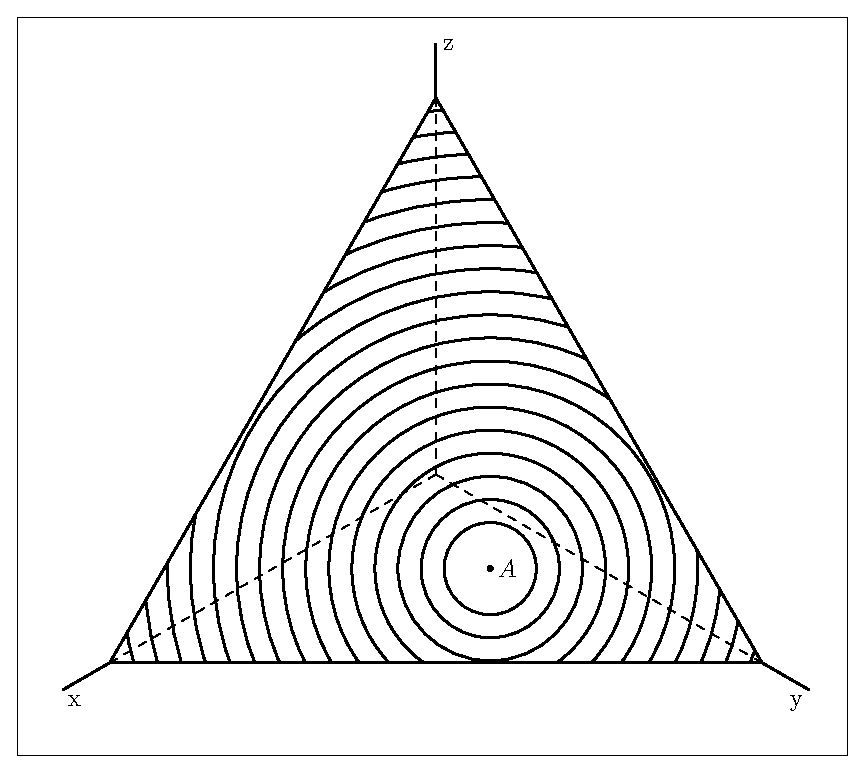
\includegraphics[width=\textwidth]{contourslp.eps}
      \caption{\footnotesize The simplex $\mathbb{S}^{2}$ in
        three-dimensional space $\mathbb{R}^{3}$ with contour lines
        corresponding to the geometry of reason around point $A$ in
        equation (\ref{eq:e6}). Points on the same contour line are
        equidistant from $A$ with respect to the Euclidean metric.
        Compare the contour lines here to figure
        \ref{fig:contoursrj}. Note that this diagram and all the
        following diagrams are frontal views of the simplex.}
      \label{fig:contourslp}
    \end{minipage}
  \end{flushright}
\end{figure}

\begin{figure}[H]
  \begin{flushright}
    \begin{minipage}[h]{.7\linewidth}
      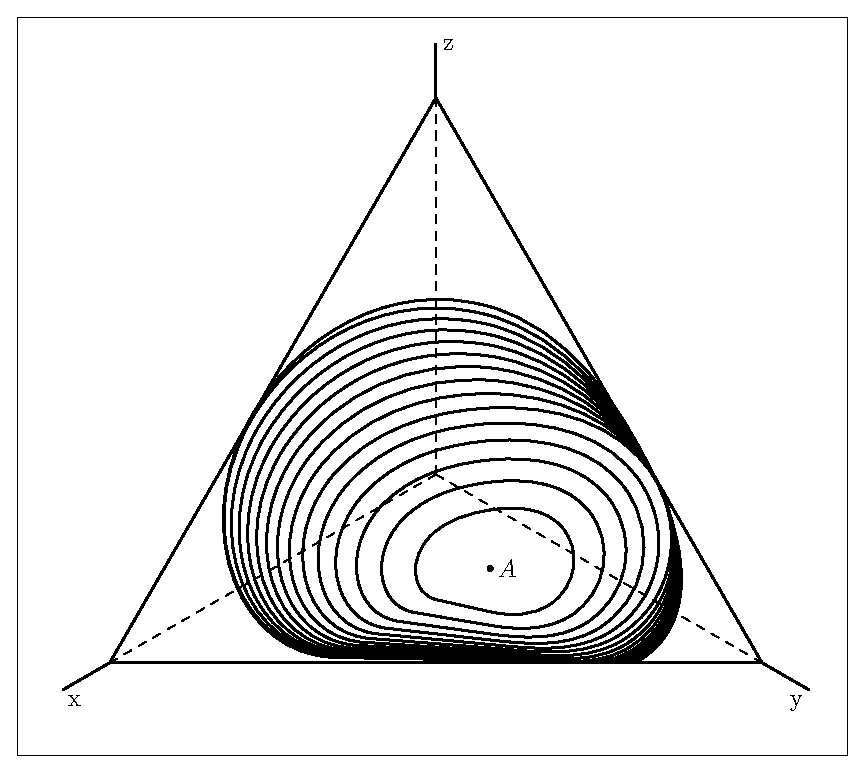
\includegraphics[width=\textwidth]{crj.eps}
      \caption{\footnotesize The simplex $\mathbb{S}^{2}$ with contour
        lines corresponding to information theory around point $A$ in
        equation (\ref{eq:e6}). Points on the same contour line are
        equidistant from $A$ with respect to the Kullback-Leibler
        divergence. The contrast to figure \ref{fig:contourslp} will
        become clear in much more detail in the body of the paper.
        Note that the contour lines of the geometry of reason are
        insensitive to the boundaries of the simplex, while the
        contour lines of information theory reflect them. One of the
        main arguments in this paper is that information theory
        respects epistemic intuitions we have about asymmetry:
        proximity to extreme beliefs with very high or very low
        probability influences the topology that is at the basis of
        updating.}
      \label{fig:contoursrj}
    \end{minipage}
  \end{flushright}
\end{figure}

\subsection{Jeffrey-Type Updating Scenarios}
\label{subsec:aixoezae}

Consider the following example of a Jeffrey-type updating scenario.

\begin{example}[Holmes]
  \label{ex:holmes}
  Sherlock Holmes attributes the following probabilities to the
  propositions $E_{i}$ that $k_{i}$ is the culprit in a crime:
  $P(E_{1})=1/3,P(E_{2})=1/2,P(E_{3})=1/6$, where $k_{1}$ is Mr.\ R.,
  $k_{2}$ is Ms.\ S., and $k_{3}$ is Ms.\ T. Then Holmes finds some
  evidence which convinces him that $P'(F^{*})=1/2$, where $F^{*}$ is
  the proposition that the culprit is male and $P$ is relatively prior
  to $P'$. What should be Holmes' updated probability that Ms.\ S. is
  the culprit?
\end{example}

I will look at the recommendations of Jeffrey conditioning and LP
conditioning for {\xample} \ref{ex:holmes} in the next section. For
now note that LP conditioning violates all of the following plausible
expectations for updating methods in Jeffrey-type updating scenarios.
This is \textbf{List A}:

\begin{itemize}
\item \textsc{continuity} An updating method ought to be continuous with
  standard conditioning as a limiting case.
\item \textsc{regularity} An updating method ought not to assign a posterior
  probability of $0$ to an event which has a positive prior
  probability and about which the intervening evidence says nothing
  except that a strictly weaker event has a positive posterior
  probability.
\item \textsc{levinstein} An updating method ought not to give
  \qeins{extremely unattractive} results in a Levinstein scenario (see
  \scite{7}{levinstein12}{}, where Benjamin Levinstein not only
  articulates this failed expectation for LP conditioning, but also
  the previous two; the following three are original to this article).
\item \textsc{invariance} An updating method ought to be partition
  invariant in the sense that introducing irrelevant subpartitioning
  does not change the outcome of the update.
\item \textsc{expansibility} An updating method ought to be insensitive to an
  expansion of the event space by zero-probability events.
\item \textsc{horizon} An updating method ought to exhibit the horizon effect
  which makes probability distributions which are nearer to extreme
  probability distributions appear to be closer to each other than
  they really are.
\end{itemize}

Jeffrey conditioning and LP conditioning are both an updating method
based on a concept of quantitative difference between probability
distributions. Evidence appears in the form of a constraint on
acceptable probability distributions and the closest acceptable
probability to the original (relatively prior) probability
distribution is chosen as its successor. Here is \textbf{List
  B}\label{page:listtwo}, a list of reasonable expectations one may
have toward this concept of quantitative difference (we call it a
distance function for the geometry of reason and a divergence for
information theory). Let $d(p,q)$ express this concept mathematically.

\begin{itemize}
\item \textsc{triangularity} The concept obeys the triangle
  inequality. If there is an intermediate probability distribution, it
  will not make the difference smaller: $d(p,r)\leq{}d(p,q)+d(q,r)$.
  Buying a pair of shoes is not going to be more expensive than buying
  the two shoes individually.
\item \textsc{collinear horizon} This expecation is just a more
  technical restatement of the \textsc{horizon} expectation in the
  previous list. If $p,p',q,q'$ are collinear with the centre of the
  simplex $m$ (whose coordinates are $m_{i}=1/n$ for all $i$) and an
  arbitrary but fixed boundary point $\xi\in\partial\mathbb{S}^{n-1}$
  and $p,p',q,q'$ are all between $m$ and $\xi$ with
  $\|p'-p\|=\|q'-q\|$ where $p$ is strictly closest to $m$, then
  $|d(p,p')|<|d(q,q')|$. For an illustration of this expectation see
  figure \ref{fig:conditions}. 
\item \textsc{transitivity of asymmetry} An ordered pair $(p,q)$ of
  simplex points associated with probability distributions is
  asymmetrically negative, positive, or balanced, so either
  $d(p,q)-d(q,p)<0$ or $d(p,q)-d(q,p)>0$ or $d(p,q)-d(q,p)=0$. If
  $(p,q)$ and $(q,r)$ are asymmetrically positive, $(p,r)$ ought not
  to be asymmetrically negative. Think of a bicycle route map with
  different locations at varying altitudes. If it takes 20 minutes to
  get from $A$ to $B$ but only 15 minutes to get from $B$ to $A$ then
  $(A,B)$ is asymmetrically positive. If $(A,B)$ and $(B,C)$ are
  asymmetrically positive, then $(A,C)$ ought not to be asymmetrically
  negative.
\end{itemize}

\begin{figure}[H]
  \begin{flushright}
    \begin{minipage}[h]{.7\linewidth}
      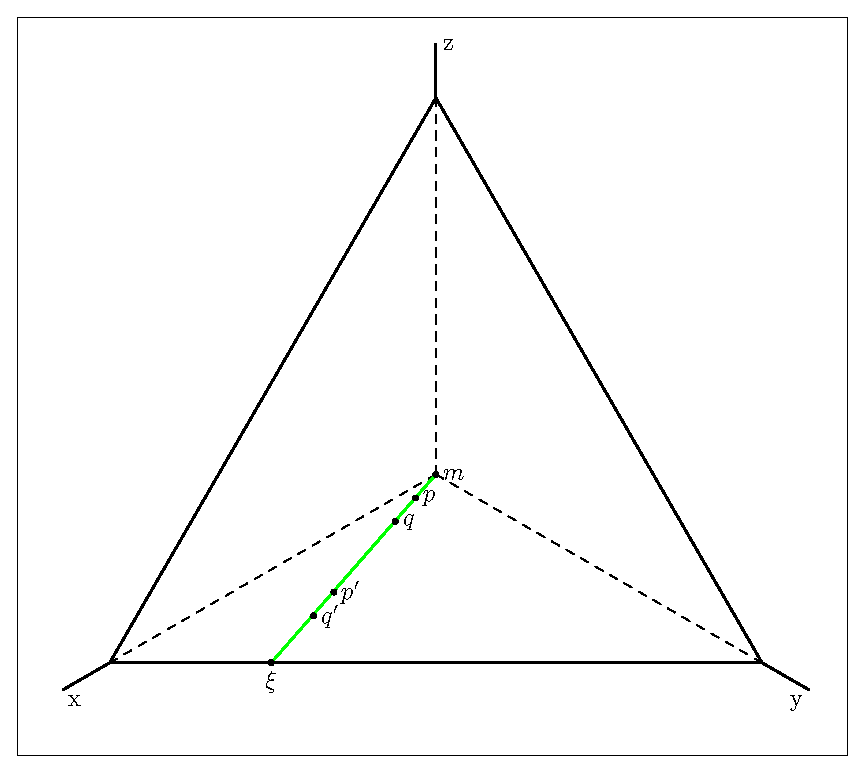
\includegraphics[width=\textwidth]{horeff.eps}
      \caption{\footnotesize An illustrations of conditions (i)--(iii)
        for \textsc{collinear horizon} in \textbf{List B}. $p,p'$ and $q,q'$
        must be equidistant and collinear with $m$ and $\xi$. If
        $q,q'$ is more peripheral than $p,p'$, then \textsc{collinear
          horizon} requires that $|d(p,p')|<|d(q,q')|$.}
      \label{fig:conditions}
    \end{minipage}
  \end{flushright}
\end{figure}

While the Kullback-Leibler divergence of information theory fulfills
all the expectations of \textbf{List A}, save \textsc{horizon}, it
fails all the expectations in \textbf{List B}. Conversely, the
Euclidean distance of the geometry of reason fulfills all the
expectations of \textbf{List B}, save \textsc{collinear horizon}, and
fails all the expectations in \textbf{List A}.

Information theory has its own axiomatic approach to justifying
standard conditioning (see \scite{7}{shorejohnson80}{}); it also
provides a justification for Jeffrey conditioning and generalizes it
(see \scite{7}{lukits15}{}). All of these virtues stand in contrast to
the violations of the expectations in \textbf{List B}. The rest of
this paper fills in the details of these violations both for the
geometry of reason and information theory, with the conclusion that
the case for the geometry of reason is hopeless while the case for
information theory is now a major challenge for future research
projects.

\subsection{LP Versus Jeffrey Conditioning}
\label{subsec:coobohcu}

Here is a simple example corresponding to example~\ref{ex:holmes}
(Sherlock Holmes) where the distance of geometry and the divergence of
information theory differ. With this difference in mind, I will show
how LP conditioning fails the expectations outlined in \textbf{List
  A}. Consider the following three points in three-dimensional space:

\begin{equation}
  \label{eq:e6}
    a=\left(\frac{1}{3},\frac{1}{2},\frac{1}{6}\right) \hspace{.5in}
    b=\left(\frac{1}{2},\frac{3}{8},\frac{1}{8}\right)  \hspace{.5in}
    c=\left(\frac{1}{2},\frac{5}{12},\frac{1}{12}\right).
\end{equation}

All three are elements of the simplex $\mathbb{S}^{2}$: their
coordinates add up to $1$. Thus they represent probability
distributions $A,B,C$ over a partition of the event space into three
mutually exclusive events. Now call $D_{\mbox{\tiny KL}}(B,A)$ the
Kullback-Leibler divergence of $B$ from $A$ defined as follows, where
$a_{i}$ are the Cartesian coordinates of $a$ (the base of the
logarithm is not important, in order to facilitate easy
differentiation I will use the natural logarithm):

\begin{equation}
  \label{eq:e7}
  D_{\mbox{\tiny KL}}(B,A)=\sum_{i=1}^{3}b_{i}\log\frac{b_{i}}{a_{i}}.
\end{equation}

Note that the Kullback-Leibler divergence, irrespective of dimension,
is always positive as a consequence of Gibbs' inequality (see
\scite{7}{mackay03}{}, sections 2.6 and 2.7).

The Euclidean distance is defined as follows:

\begin{equation}
  \label{eq:e3}
  \|B-A\|=\sqrt{\sum_{i=1}^{n}\left(b_{i}-a_{i}\right)^{2}}.
\end{equation}

What is remarkable about the three points in (\ref{eq:e6}) is that

\begin{equation}
  \label{eq:e8}
  \|C-A\|\approx{}0.204<\|B-A\|\approx{}0.212
\end{equation}

and

\begin{equation}
  \label{eq:e9}
  D_{\mbox{\tiny KL}}(B,A)\approx{}0.0589<D_{\mbox{\tiny KL}}(C,A)\approx{}0.069.
\end{equation}

The Kullback-Leibler divergence and Euclidean distance give different
re\-commendations with respect to proximity. In terms of the global
inaccuracy measure presented in Leitgeb and Pettigrew (see
\scite{8}{leitgebpettigrew10i}{206}) and $E=W$ (all possible worlds
are epistemically accessible),

\begin{equation}
  \label{eq:e8a}
  \mbox{GExp}_{A}(C)\approx{}0.653<\mbox{GExp}_{A}(B)\approx{}0.656.
\end{equation}

Global inaccuracy reflects the Euclidean proximity relation, not the
re\-commendation of information theory. If $A$ corresponds to my prior
and my evidence is such that I must change the first coordinate to
$1/2$ (as in {\xample}~\ref{ex:holmes} about Sherlock Holmes) and
nothing stronger, then information theory via the Kullback-Leibler
divergence re\-commends the posterior corresponding to $B$; the
geometry of reason as expounded in Leitgeb and Pettigrew recommends
the posterior corresponding to $C$.

Here is a brief account of Jeffrey conditioning and LP conditioning,
which are competing methods to arrive at posterior probability
distributions in Jeffrey-type updating scenarios. They roughly align
with information theory and the geometry of reason, respectively, in
the context of this paper. There are, however, many formal
epistemologists who defend the epistemic norm of Jeffrey conditioning
but are skeptical about further claims of information theory, such as
updating in scenarios that pose an affine constraint which are not
Jeffrey-type updating scenarios, for example Bas van Fraassen's Judy
Benjamin problem (see van Fraassen, \scite{11}{fraassen81}{}; for the
debate over information theory and affine constraints see
\scite{7}{lukits14}{}).

\begin{example}[Abstract Holmes]
  \label{ex:abstract}
  Consider a possibility space $W=E_{1}\cup{}E_{2}\cup{}E_{3}$ (the
  $E_{i}$ are sets of states which are pairwise disjoint and whose
  union is $W$) and a partition $\mathcal{F}$ of $W$ such that
  $\mathcal{F}=\{F^{*},F^{**}\}=\{E_{1},E_{2}\cup{}E_{3}\}$.
\end{example}

Let $P$ be the prior probability function on $W$ and $P'$ the
posterior. I will keep the notation informal to make this simple, not
mathematically precise. Jeffrey-type updating scenarios give us new
information on the posterior probabilities of partitions such as
$\mathcal{F}$. In {\xample} \ref{ex:abstract}, let

\begin{equation}
  \label{eq:priors}
  \begin{array}{rcl}
    P(E_{1})&=&1/3 \\
    P(E_{2})&=&1/2 \\
    P(E_{3})&=&1/6
  \end{array}
\end{equation}

and the new evidence constrain $P'$ such that
$P'(F^{*})=1/2=P'(F^{**})$.

Jeffrey conditioning works on the following intuition, which elsewhere
I have called Richard Jeffrey's updating principle \textsc{jup} (see
also \scite{7}{wagner02}{}). The posterior probabilities conditional
on the partition elements equal the prior probabilities conditional on
the partition elements since we have no information in the evidence
that they should have changed. Hence,

\begin{align}
  \label{eq:jc}
  &P'_{\mbox{\tiny JC}}(E_{i})&=&P'(E_{i}|F^{*})P'(F^{*})+P'(E_{i}|F^{**})P'(F^{**})\notag \\
  &&=&P(E_{i}|F^{*})P'(F^{*})+P(E_{i}|F^{**})P'(F^{**})
\end{align}

Jeffrey conditioning is controversial (for an introduction to Jeffrey
conditioning see \scite{7}{jeffrey65}{}; for its statistical and
formal properties see \scite{7}{diaconiszabell82}{}; for a pragmatic
vindication of Jeffrey conditioning see \scite{7}{armendt80}{}, and
\scite{7}{skyrms86}{}; for criticism see
\scite{7}{howsonfranklin94}{}). Information theory, however, supports
Jeffrey conditioning. Leitgeb and Pettigrew show that Jeffrey
conditioning does not in general pick out the minimally inaccurate
posterior probability distribution, given their assumptions. If the
geometry of reason as presented in Leitgeb and Pettigrew is sound,
this would constitute a powerful criticism of Jeffrey conditioning.
Leitgeb and Pettigrew introduce an alternative to Jeffrey conditioning
(LP conditioning). It proceeds as follows for {\xample}
\ref{ex:abstract} and in general provides the minimally inaccurate
posterior probability distribution in Jeffrey-type updating scenarios
according to the geometry of reason.

Solve the following two equations for $x$ and $y$:

\begin{equation}
  \label{eq:lpce}
  \begin{array}{rcl}
    P(E_{1})+x&=&P'(F^{*}) \\
    P(E_{2})+y+P(E_{3})+y&=&P'(F^{**})
  \end{array}
\end{equation}

and then set

\begin{equation}
  \label{eq:lpcf}
  \begin{array}{rcl}
    P'_{\mbox{\tiny LP}}(E_{1})&=&P(E_{1})+x \\
    P'_{\mbox{\tiny LP}}(E_{2})&=&P(E_{2})+y \\
    P'_{\mbox{\tiny LP}}(E_{3})&=&P(E_{3})+y
  \end{array}
\end{equation}

For the more formal and more general account see
\scite{8}{leitgebpettigrew10ii}{254}. The results for {\xample}
\ref{ex:abstract} are:

\begin{equation}
  \label{eq:lpcres}
  \begin{array}{rcl}
    P'_{\mbox{\tiny LP}}(E_{1})&=&1/2 \\
    P'_{\mbox{\tiny LP}}(E_{2})&=&5/12 \\
    P'_{\mbox{\tiny LP}}(E_{3})&=&1/12
  \end{array}
\end{equation}

Compare these results to the results of Jeffrey conditioning:

\begin{equation}
  \label{eq:jcres}
  \begin{array}{rcl}
    P'_{\mbox{\tiny JC}}(E_{1})&=&1/2 \\
    P'_{\mbox{\tiny JC}}(E_{2})&=&3/8 \\
    P'_{\mbox{\tiny JC}}(E_{3})&=&1/8
  \end{array}
\end{equation}

Note that (\ref{eq:priors}), (\ref{eq:jcres}), and (\ref{eq:lpcres})
correspond to $A,B,C$ in (\ref{eq:e6}) (see
{\igure}~\ref{fig:threepoints}).

\begin{figure}[H]
  \begin{flushright}
    \begin{minipage}[h]{.7\linewidth}
      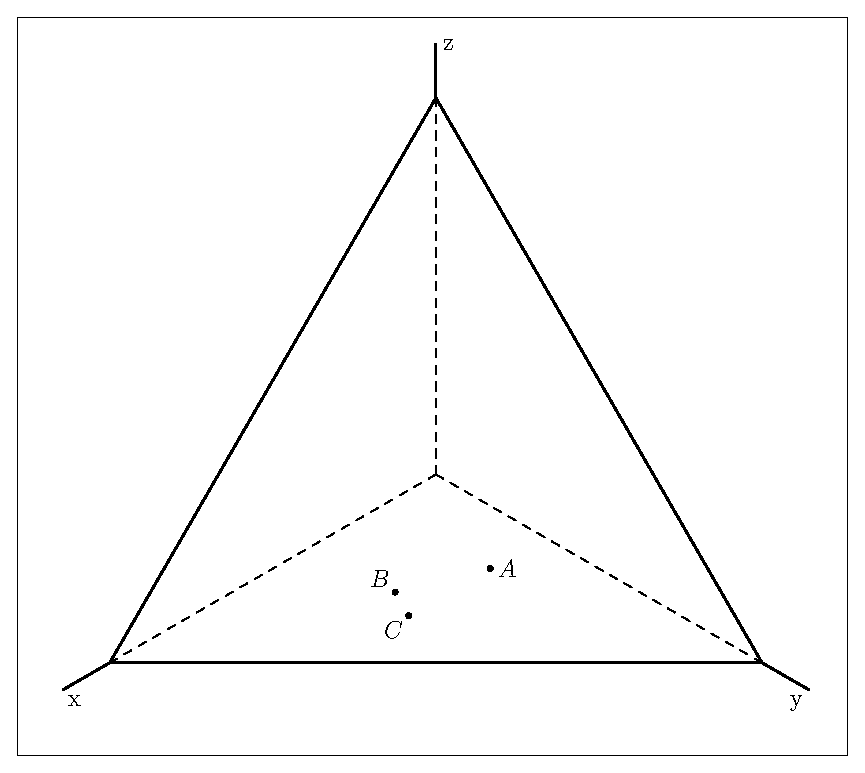
\includegraphics[width=\textwidth]{threepoints.eps}
      \caption{\footnotesize The simplex $\mathbb{S}^{2}$ in
        three-dimensional space $\mathbb{R}^{3}$ with points $a,b,c$
        as in equation (\ref{eq:e6}) representing probability
        distributions $A,B,C$. Note that geometrically speaking $C$ is
        closer to $A$ than $B$ is. Using the Kullback-Leibler
        divergence, however, $B$ is closer to $A$ than $C$ is.}
      \label{fig:threepoints}
    \end{minipage}
  \end{flushright}
\end{figure}

\subsection{Expectation Violations for the Geometry of Reason}
\label{subsec:zoocaesh}

This subsection provides more detail for the expectations in \textbf{List
  A} and shows how LP conditioning violates them.

\subsubsection{Continuity}
\label{Continuity}

LP conditioning violates \textsc{continuity} because standard
conditioning gives a different recommendation than LP conditioning
when they are used in a scenario where both are applicable. 
% a parallel sequence of Jeffrey-type updating scenarios which get
% arbitrarily close to standard event observation.
This is troubling considering how important fulfilling
\textsc{conditioning} (the requirement in
{\ubsection}~\ref{subsec:ayudoosa}) is to Leitgeb and Pettigrew.

% To illustrate a \textsc{continuity} violation, consider the case where
% Sherlock Holmes reduces his credence that the culprit was male to
% $\varepsilon_{n}=1/n$ for $n=4,5,\ldots$. The sequence
% $\varepsilon_{n}$ is not meant to reflect a case where Sherlock Holmes
% becomes successively more certain that the culprit was female. It is
% meant to reflect countably many parallel scenarios which only differ
% by the degree to which Sherlock Holmes is sure that the culprit was
% female. These parallel scenarios give rise to a parallel sequence (as
% opposed to a successive sequence) of updated probabilities
% $P'_{\mbox{\tiny LP}}(F^{**})$ and another sequence of updated
% probabilities $P'_{\mbox{\tiny JC}}(F^{**})$ ($F^{**}$ is the
% proposition that the culprit is female). As $n\rightarrow\infty$, both
% of these sequences go to one.

To illustrate a \textsc{continuity} violation, consider the prior
probabilities in {\xample} \ref{ex:holmes} and the case where Sherlock
Holmes becomes certain that the culprit is female. Straightforward
conditionalization results in 

\begin{equation}
  \label{eq:sherlockcontsc}
  \begin{array}{rcl}
  P'_{\mbox{\tiny SC}}(E_{1})&=&0\\
  P'_{\mbox{\tiny SC}}(E_{2})&=&3/4\\
  P'_{\mbox{\tiny SC}}(E_{3})&=&1/4
\end{array}
\end{equation}

% Letting $n\rightarrow\infty$ for Jeffrey conditioning yields

% \begin{equation}
%   \label{eq:sherlockcontjc}
%   \begin{array}{rcccl}
%   P'_{\mbox{\tiny JC}}(E_{1})&=&1/n&\rightarrow&0\\
%   P'_{\mbox{\tiny JC}}(E_{2})&=&3(n-1)/4n&\rightarrow&3/4\\
%   P'_{\mbox{\tiny JC}}(E_{3})&=&(n-1)/4n&\rightarrow&1/4
% \end{array}
% \end{equation}

% whereas letting $n\rightarrow\infty$ for 

LP conditioning yields

% \begin{equation}
%   \label{eq:sherlockcontlp}
%   \begin{array}{rcccl}
%   P'_{\mbox{\tiny LP}}(E_{1})&=&1/n&\rightarrow&0\\
%   P'_{\mbox{\tiny LP}}(E_{2})&=&(4n-3)/6n&\rightarrow&2/3\\
%   P'_{\mbox{\tiny LP}}(E_{3})&=&(2n-5)/6n&\rightarrow&1/3
% \end{array}
% \end{equation}

\begin{equation}
  \label{eq:sherlockcontlp}
  \begin{array}{rcl}
  P'_{\mbox{\tiny LP}}(E_{1})&=&0\\
  P'_{\mbox{\tiny LP}}(E_{2})&=&2/3\\
  P'_{\mbox{\tiny LP}}(E_{3})&=&1/3
\end{array}
\end{equation}

LP conditioning violates \textsc{continuity}.

\subsubsection{Regularity}
\label{Regularity}

LP conditioning violates \textsc{regularity} because formerly positive
probabilities can be reduced to $0$ even though the new information in
the Jeffrey-type updating scenario makes no such requirements (as is
usually the case for standard conditioning). Ironically, Jeffrey-type
updating scenarios are meant to be a better reflection of real-life
updating because they avoid extreme probabilities (see
\scite{7}{jeffrey87}{}).

The violation becomes serious if we are already sympathetic to an
infor\-ma\-tion-based account: the amount of information required to turn
a non-extreme probability into one that is extreme ($0$ or $1$) is
infinite. Whereas the geometry of reason considers extreme
probabilities to be easily accessible by non-extreme probabilities
under new information (much like a marble rolling off a table or a
bowling ball heading for the gutter), information theory envisions
extreme probabilities more like an event horizon. The nearer you are
to the extreme probabilities, the more information you need to move
on. For an observer, the horizon is never reached.

% \begin{quotex}
%   \beispiel{Regularity Holmes}\label{ex:regularity} Everything is as
%   in {\xample} \ref{ex:holmes}, except that Sherlock Holmes becomes
%   confident to a degree of $2/3$ that Mr.\ R is the culprit and
%   updates his relatively prior probability distribution in
%   (\ref{eq:priors}).
% \end{quotex}

\begin{example}[Regularity Holmes]
  \label{ex:regularity}
  Everything is as in {\xample} \ref{ex:holmes}, except that Sherlock
  Holmes becomes confident to a degree of $2/3$ that Mr.\ R is the
  culprit and updates his relatively prior probability distribution in
  (\ref{eq:priors}).
\end{example}

Then his posterior probabilities look as follows:

\begin{equation}
  \label{eq:sherlockposteriorjcreg}
  \begin{array}{rcl}
  P'_{\mbox{\tiny JC}}(E_{1})&=&2/3\\
  P'_{\mbox{\tiny JC}}(E_{2})&=&1/4\\
  P'_{\mbox{\tiny JC}}(E_{3})&=&1/12
\end{array}
\end{equation}

\begin{equation}
  \label{eq:sherlockposteriorlpreg}
  \begin{array}{rcl}
  P'_{\mbox{\tiny LP}}(E_{1})&=&2/3\\
  P'_{\mbox{\tiny LP}}(E_{2})&=&1/3\\
  P'_{\mbox{\tiny LP}}(E_{3})&=&0
\end{array}
\end{equation}

With LP conditioning, Sherlock Holmes' subjective probability that
Ms.\ T is the culprit in {\xample} \ref{ex:regularity} has been reduced
to zero. 
% No finite amount of information could bring Ms.\ T back into
% consideration as a culprit in this crime, and Sherlock Holmes should
% be willing to bet any amount of money against a penny that she is not
% the culprit---even though his evidence is nothing more than an
% increase in the probability that Mr.\ R is the culprit.
LP conditioning violates \textsc{regularity}.

\subsubsection{Levinstein}
\label{Levinstein}

LP conditioning violates \textsc{levinstein} because of \qeins{the
  potentially dramatic effect [LP conditioning] can have on the
  likelihood ratios between different propositions}
\scite{3}{levinstein12}{419}. Consider Levinstein's example:

% \begin{quotex}
%   \beispiel{Levinstein's Ghost}\label{ex:levinstein} There is a car
%   behind an opaque door, which you are almost sure is blue but which
%   you know might be red. You are almost certain of materialism, but
%   you admit that there's some minute possibility that ghosts exist.
%   Now the opaque door is opened, and the lighting is fairly good. You
%   are quite surprised at your sensory input: your new credence that
%   the car is red is very high.
% \end{quotex}

\begin{example}[Levinstein's Ghost]
  \label{ex:levinstein}
  There is a car behind an opaque door, which you are almost sure is
  blue but which you know might be red. You are almost certain of
  materialism, but you admit that there's some minute possibility that
  ghosts exist. Now the opaque door is opened, and the lighting is
  fairly good. You are quite surprised at your sensory input: your new
  credence that the car is red is very high.
\end{example}

Jeffrey conditioning leads to no change in opinion about ghosts. Under
LP conditioning, however, seeing the car raises the probability that
there are ghosts to an astonishing 47\%, given Levinstein's reasonable
priors. Levinstein proposes a logarithmic inaccuracy measure as a
remedy to avoid violation of \textsc{levinstein}. As a special case of
applying a Levinstein-type logarithmic inaccuracy measure, information
theory does not violate \textsc{levinstein}.

\subsubsection{Invariance}
\label{Invariance}

LP conditioning violates \textsc{invariance} because two agents who
have identical credences with respect to a partition of the event
space may disagree about this partition after LP conditioning, even
when the Jeffrey-type updating scenario provides no new information
about the more finely grained partitions on which the two agents
disagree. In the following example, Sherlock Holmes and Jane Marple
agree on all relevant facts and on their prior probabilities, but LP
conditioning leads to a divergence in posterior probabilities.

\begin{example}[Jane Marple]
  \label{ex:marple}
  Jane Marple is on the same case as Sherlock Holmes in {\xample}
  \ref{ex:holmes} and arrives at the same relatively prior probability
  distribution as Sherlock Holmes (I will call Jane Marple's
  relatively prior probability distribution $Q$ and her posterior
  probability distribution $Q'$). Jane Marple, however, has a more
  finely grained probability assignment than Sherlock Holmes and
  distinguishes between the case where Ms.\ S went to boarding school
  with her, of which she has a vague memory, and the case where Ms.\ S
  did not and the vague memory is only about a fleeting resemblance of
  Ms.\ S with another boarding school mate. Whether or not Ms.\ S went
  to boarding school with Jane Marple is completely beside the point
  with respect to the crime, and Jane Marple considers the
  possibilities equiprobable whether or not Ms.\ S went to boarding
  school with her.
\end{example}

Let $E_{2}\equiv{}E_{2}^{*}\vee{}E_{2}^{**}$, where $E_{2}^{*}$ is the
proposition that Ms.\ S is the culprit and she went to boarding school
with Jane Marple and $E_{2}^{**}$ is the proposition that Ms.\ S is
the culprit and she did not go to boarding school with Jane Marple.
Then

\begin{equation}
  \label{eq:marpleprior}
  \begin{array}{rcl}
  Q(E_{1})&=&1/3\\
  Q(E_{2}^{*})&=&1/4\\
  Q(E_{2}^{**})&=&1/4\\
  Q(E_{3})&=&1/6
\end{array}
\end{equation}

Now note that while Sherlock Holmes and Jane Marple agree on the
relevant facts of the criminal case (who is the culprit?) in their
posterior probabilities if they use Jeffrey conditioning,

\begin{equation}
  \label{eq:sherlockposteriorjc}
  \begin{array}{rcl}
  P'_{\mbox{\tiny JC}}(E_{1})&=&1/2\\
  P'_{\mbox{\tiny JC}}(E_{2})&=&3/8\\
  P'_{\mbox{\tiny JC}}(E_{3})&=&1/8
\end{array}
\end{equation}

\begin{equation}
  \label{eq:marpleposteriorjc}
  \begin{array}{rcl}
  Q'_{\mbox{\tiny JC}}(E_{1})&=&1/2\\
  Q'_{\mbox{\tiny JC}}(E_{2}^{*})&=&3/16\\
  Q'_{\mbox{\tiny JC}}(E_{2}^{**})&=&3/16\\
  Q'_{\mbox{\tiny JC}}(E_{3})&=&1/8
\end{array}
\end{equation}

they do not agree if they use LP conditioning,

\begin{equation}
  \label{eq:sherlockposteriorlp}
  \begin{array}{rcl}
  P'_{\mbox{\tiny LP}}(E_{1})&=&1/2\\
  P'_{\mbox{\tiny LP}}(E_{2})&=&5/12\\
  P'_{\mbox{\tiny LP}}(E_{3})&=&1/12
\end{array}
\end{equation}

\begin{equation}
  \label{eq:marpleposteriorlp}
  \begin{array}{rcl}
  Q'_{\mbox{\tiny LP}}(E_{1})&=&1/2\\
  Q'_{\mbox{\tiny LP}}(E_{2}^{*})&=&7/36\\
  Q'_{\mbox{\tiny LP}}(E_{2}^{**})&=&7/36\\
  Q'_{\mbox{\tiny LP}}(E_{3})&=&1/9
\end{array}
\end{equation}

Selten, a defender of the Brier score against the Log score, uses the
label \qnull{elongation invariance} for \textsc{invariance}. LP
conditioning violates \textsc{invariance}.

\subsubsection{Expansibility}
\label{Expansibility}

One particular problem with the lack of invariance for LP conditioning
is how zero-probability events should be included in the list of prior
probabilities that determines the value of the posterior
probabilities. Consider

\begin{equation}
  \label{eq:reginvone}
  \begin{array}{rcl}
  P(X_{1})&=&0\\
  P(X_{2})&=&0.3\\
  P(X_{3})&=&0.6\\
  P(X_{4})&=&0.1\\
\end{array}
\end{equation}

That $P(X_{1})=0$ may be a consequence of standard conditioning in a
previous step. Now the agent learns that $P'(X_{3}\vee{}X_{4})=0.5$.
Should the agent update on the list presented in (\ref{eq:reginvone})
or on the following list:

\begin{equation}
  \label{eq:reginvtwo}
  \begin{array}{rcl}
  P(X_{2})&=&0.3\\
  P(X_{3})&=&0.6\\
  P(X_{4})&=&0.1\\
\end{array}
\end{equation}

Whether you update on (\ref{eq:reginvone}) or (\ref{eq:reginvtwo})
makes no difference to Jeffrey conditioning, but due to the lack of
invariance it makes a difference to LP conditioning, so the geometry
of reason needs to find a principled way to specify the appropriate
prior probabilities. The only non-arbitrary way to do this is either
to include or to exclude all zero probability events on the list. This
strategy, however, sounds ill-advised unless one signs on to a
stronger version of \textsc{regularity} and requires that only a fixed
set of events can have zero probabilities (such as logical
contradictions), but the geometry of reason is joined at the hip with
LP conditioning which runs afoul of \textsc{regularity} even when it
updates on priors and evidence that obey \textsc{regularity} (see
{\ubsection}~\ref{Regularity}).

LP conditioning violates \textsc{expansibility}. Selten has a
requirement for scoring rules similar to \textsc{expansibility} that
he calls elongation invariance (axiom 2 in \scite{8}{selten98}{54}).
It is to some degree ironic that Selten uses elongation invariance to
show that the Brier score and its close relatives are the only
reasonable scoring rules, when a decade later Leitgeb and Pettigrew
derive an updating method from the geometry of reason so intimately
associated with the Brier score that violates an immediate analogy to
Selten's elongation invariance.

\subsubsection{Horizon}
\label{Horizon}

\begin{example}[Undergraduate Complaint]
  \label{ex:complaint}
  An undergraduate student complains to the department head that the
  professor will not reconsider an 89\% grade (which misses an A+ by
  one percent) when reconsideration was given to other students with a
  67\% grade (which misses a B- by one percent).
\end{example}

Intuitions may diverge, but the professor's reasoning is as follows.
To improve a 60\% paper by ten percent is easily accomplished: having
your roommate check your grammar, your spelling, and your line of
argument will sometimes do the trick. It is incomparably more
difficult to improve an 85\% paper by ten percent: it may take doing a
PhD to turn a student who writes the former into a student who writes
the latter. A maiore ad minus, the step from 89\% to 90\% is greater
than the step from 67\% to 68\%.

Another example for the horizon effect is George Schlesinger's
comparison between the risk of a commercial airplane crash and the
risk of a military glider landing in enemy territory.

\begin{example}[Airplane Gliders]
  \label{ex:schlesinger}
  Compare two scenarios. In the first, an airplane which is considered
  safe (probability of crashing is $1/10^{9}$) goes through an
  inspection where a mechanical problem is found which increases the
  probability of a crash to $1/100$. In the second, military gliders
  land behind enemy lines, where their risk of perishing is 26\%. A
  slight change in weather pattern increases this risk to 27\%.
  \scite{3}{schlesinger95}{211}
\end{example}

I claim that an updating method ought to fulfill the requirements of
the horizon effect: it ought to be more difficult to update as
probabilities become more extreme (or less middling). I have
formalized this requirement in \textbf{List B}. It is trivial that the
geometry of reason does not fulfill it. Information theory fails as
well, which gives the horizon effect its prominent place in both
lists. The way information theory fails, however, is quite different.
Near the boundary of $\mathbb{S}^{n-1}$, information theory reflects
the horizon effect just as our expectation requires. The problem is
near the centre, where some points are more divergent the closer they
are to the middle. I will give an example and more explanation in
{\ubsection}~\ref{subsubsec:colhor}.

\subsection{Expectations for Information Theory}
\label{subsec:expinfth}

In information theory, the information loss differs depending on
whether one uses probability distribution $P$ to encode a message
distributed according to probability distribution $Q$, or whether one
uses probability distribution $Q$ to encode a message distributed
according to probability distribution $P$. This asymmetry may very
well carry over into the epistemic realm. Updating from one
probability distribution, for example, which has $P(X)=x>0$ to
$P'(X)=0$ is common. Going in the opposite direction, however, from
$P(X)=0$ to $P'(X)=x'>0$ is controversial and unusual.

Associated with the Log score via McCarthy's theorem
({\heorem}~\ref{thm:lahpoodu}) is the Kullback-Leibler divergence,
which is the most promising concept of difference for probability
distributions in information theory and the one which gives us
Bayesian standard conditioning as well as Jeffrey conditioning. It is
non-commutative and may provide the kind of asymmetry required to
reflect epistemic asymmetry. However, it also violates
\textsc{triangularity}, \textsc{collinear horizon}, and
\textsc{transitivity of asymmetry}. The task of this section is to
show how serious these violations are.

\subsubsection{Triangularity}
\label{subsubsec:triangularity}

There is an interesting connection between LP conditioning and Jeffrey
conditioning as updating methods. Let $B$ be on the zero-sum line
between $A$ and $C$ if and only if

\begin{equation}
\label{eq:jooziphu}
d(A,C)=d(A,B)+d(B,C),
\end{equation}

where $d$ is the difference measure we are using, so $d(A,B)=\|B-A\|$
for the geometry of reason and $d(A,B)=D_{\mbox{\tiny KL}}(B,A)$ for
information geometry. For the geometry of reason (and Euclidean
geometry), the zero-sum line between two probability distributions is
just what we intuitively think of as a straight line: in Cartesian
coordinates, $B$ is on the zero-sum line strictly between $A$ and $C$
if and only if for some $\vartheta\in(0,1)$,
$b_{i}=\vartheta{}a_{i}+(1-\vartheta)c_{i}$ and $i=1,\ldots,n$.

What the zero-sum line looks like for information theory is
illustrated in figure \ref{fig:eugoohue}. The reason for the oddity is
that the Kullback-Leibler divergence does not obey
\textsc{triangularity}. Call $B$ a zero-sum point between $A$ and $C$
if (\ref{eq:jooziphu}) holds true. For the geometry of reason, the
zero-sum points are simply the points on the straight line between $A$
and $C$. For information geometry, the zero-sum points are the
boundary points of the set where you can take a shortcut by making a
detour, i.e.\ all points for which $d(A,B)+d(B,C)<d(A,C)$.

\begin{figure}[H]
    \begin{minipage}[h]{.7\linewidth}
      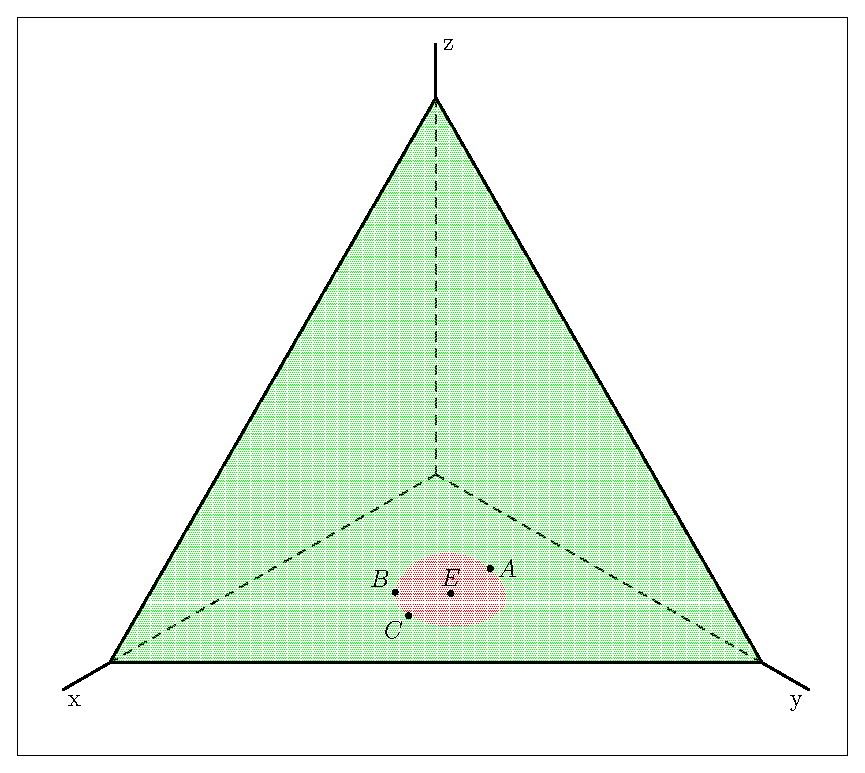
\includegraphics[width=\textwidth]{dreieck.eps}
      \caption{\footnotesize The zero-sum line between $A$ and $C$ is
        the boundary line between the green area, where the triangle
        inequality holds, and the red area, where the triangle
        inequality is violated. The posterior probability distribution
        $B$ recommended by Jeffrey conditioning always lies on the
        zero-sum line between the prior $A$ and the LP posterior $C$,
        as per equation (\ref{eq:ocidocho}). $E$ is the point in the
        red area where the triangle inequality is most efficiently
        violated. Even though it can be calculated using the Lambert W
        function,
        $e_{k}=\frac{c_{k}}{W\left(\frac{c_{k}}{a_{k}}\exp(1+\lambda)\right)}$,
        with $\lambda$ chosen to fulfill $\sum{}e_{k}=1$, it is not
        clear to me whether $E$ is the midpoint between $A$ and $C$ or
        not.}
      \label{fig:eugoohue}
\end{minipage}
\end{figure}

\begin{proposition}
    \label{prp:ozohquee}
    If $A$ represents a relatively prior probability distribution and
    $C$ the posterior probability distribution recommended by LP
    conditioning, the posterior probability distribution recommended
    by Jeffrey conditioning is always a zero-sum point with respect to
    the Kullback-Leibler divergence,
\begin{equation}
  \label{eq:ocidocho}
  D_{\mbox{\tiny KL}}(C,A)=D_{\mbox{\tiny KL}}(B,A)+D_{\mbox{\tiny KL}}(C,B).
\end{equation}
\end{proposition}

\begin{proof}
  \label{prf:chaiphah}
  To prove equation (\ref{eq:ocidocho}) in the case $n=3$ (assuming
  that LP conditioning does not \qnull{fall off the edge} as in case
  (b) in \scite{8}{leitgebpettigrew10ii}{253}) note that all three
  points (prior; point recommended by Jeffrey conditioning; and point
  recommended by LP conditioning) can be expressed using three
  variables suitably constrained to yield probabilities (for example,
  $\alpha-\beta>0$):
\begin{equation}
  \label{eq:reejeiru}
  \begin{array}{rcl}
    A&=&\left(1-\alpha,\beta,\alpha-\beta\right) \\
     && \\
    B&=&\left(1-\gamma,\frac{\gamma\beta}{\alpha},\frac{\gamma(\alpha-\beta)}{\alpha}\right) \\
     && \\
    C&=&\left(1-\gamma,\beta+\frac{1}{2}(\gamma-\alpha),\alpha-\beta+\frac{1}{2}(\gamma-\alpha)\right)
  \end{array}
\end{equation}
The rest is basic algebra using the definition of the Kullback-Leibler
divergence in (\ref{eq:e7}). 

\begin{equation}
  \label{eq:eirohzai}
  \begin{split}
  & (1-\gamma)\log\frac{1-\gamma}{1-\alpha}+\left(\beta+\frac{1}{2}(\gamma-\alpha)\right)\log\frac{\beta+\frac{1}{2}(\gamma-\alpha)}{\beta}+ \\
  & \left(\alpha-\beta+\frac{1}{2}(\gamma-\alpha)\right)\log\frac{\alpha-\beta+\frac{1}{2}(\gamma-\alpha)}{\alpha-\beta}= \\
  & (1-\gamma)\log\frac{1-\gamma}{1-\alpha}+\frac{\gamma\beta}{\alpha}\log\frac{\frac{\gamma\beta}{\alpha}}{\beta}+\frac{\gamma(\alpha-\beta)}{\alpha}\log\frac{\frac{\gamma(\alpha-\beta)}{\alpha}}{\alpha-\beta}+ \\
  & (1-\gamma)\log\frac{1-\gamma}{1-\gamma}+\left(\beta+\frac{1}{2}(\gamma-\alpha)\right)\log\frac{\beta+\frac{1}{2}(\gamma-\alpha)}{\frac{\gamma\beta}{\alpha}}+ \\
  & \left(\alpha-\beta+\frac{1}{2}(\gamma-\alpha)\right)\log\frac{\alpha-\beta+\frac{1}{2}(\gamma-\alpha)}{\frac{\gamma(\alpha-\beta)}{\alpha}}
  \end{split}
\end{equation}

In order to prove the claim for arbitrary $n$ one simply generalizes
(\ref{eq:reejeiru}).
\end{proof}

Informationally speaking, if you go from $A$ to $C$, you can just as
well go from $A$ to $B$ and then from $B$ to $C$. This does not mean
that we can conceive of information geometry the way we would conceive
of non-Euclidean geometry, where it is also possible to travel faster
on what from a Euclidean perspective looks like a detour. For in
information geometry, you can travel faster on what from the
perspective of information theory (!) looks like a detour, i.e.\ the
triangle inequality does not hold. 

Before we get carried away with these analogies between divergences
and metrics, however, it is important to note that it is not
appropriate to impose expectations that are conventional for metrics
on divergences. Bregman divergences, for example, in some sense
violate the triangle equality by design. If $d_{H}$ is a Bregman
divergence with the corresponding convex entropy function $H$, then
for a convex set $\mathcal{C}\in\mathbb{R}^{n}$ and all
$x\in{}\mathcal{C}$ and $y\in\mathbb{R}^{n}$ the following reverse
triangle inequality is true:
\begin{equation}
\label{eq:aiphaiho}
d_{H}(x,y)\geq{}d_{H}(x,y')+d_{H}(y',y), 
\end{equation}
where $y'$ is the projection of $y$ onto $\mathcal{C}$ such that
$d_{H}(y',y)=\min\{d_{H}(z,y),z\in{}\mathcal{C}\}$. The squared
Euclidean distance is an interesting case in point for this property.
In a generalization of the Pythagorean theorem, $c^{2}>a^{2}+b^{2}$
holds for obtuse triangles. When $\mathcal{C}$ is affine (such as a
plane in $\mathbb{R}^{3}$), (\ref{eq:aiphaiho}) turns from an
inequality to an equation (replacing \qnull{$\geq$} by \qnull{$=$})
for all Bregman divergences. For the squared Euclidean distance,
(\ref{eq:aiphaiho}) is then the conventional Pythagorean theorem. To
subject the difference concept between probability distributions to a
\textsc{triangularity} requirement may be a temptation to resist and
only reveal another instance of the Euclidean prejudice identified by
Mormann.

% This is false.
% It is a handy corollary of {\roposition}~\ref{prp:ozohquee} that
% whenever $(A,B)$ and $(B,C)$ violate \textsc{transitivity of
%   asymmetry} then
% \begin{equation}
%   \label{eq:saithain}
%   D_{\mbox{\tiny KL}}(A,C)>D_{\mbox{\tiny KL}}(B,C)+D_{\mbox{\tiny KL}}(A,B).
% \end{equation}

The three points $A,B,C$ in (\ref{eq:e6}) violate 
\textsc{triangularity} for $D_{\mbox{\tiny KL}}$ because
\begin{equation}
  \label{eq:yaifahge}
  0.067806=D_{\mbox{\tiny KL}}(A,B)+D_{\mbox{\tiny KL}}(B,C)<D_{\mbox{\tiny KL}}(A,C)=0.071530.
\end{equation}
Information theory, however, does not only violate
\textsc{triangularity}. It violates it in a particularly egregious
way.

\begin{proposition}
      \label{prp:yahmuthe}
      Let $x$ and $z$ be distinct points on $\mathbb{S}^{n-1}$ with
      coordinates $x_{i}$ and $z_{i}$ ($1\leq{}i\leq{}n$).
      Then, for any $\vartheta\in{}(0,1)$ and an intermediate point
      $y$ with coordinates
      $y_{i}=\vartheta{}x_{i}+(1-\vartheta)z_{i}$, the following
      inequality holds true:
\begin{equation}
  \label{eq:aiphedau}
  D_{\mbox{\tiny KL}}(z,x)>D_{\mbox{\tiny KL}}\left(y,x\right)+D_{\mbox{\tiny KL}}\left(z,y\right).
\end{equation}
\end{proposition}

\begin{proof}
    \label{prf:othahtha}
It is straightforward to see that (\ref{eq:aiphedau}) is equivalent to
\begin{equation}
  \label{eq:eiquotoh}
  \sum_{i=1}^{n}(z_{i}-x_{i})\log\frac{\vartheta{}x_{i}+(1-\vartheta)z_{i}}{x_{i}}>0.
\end{equation}
Expand the right hand side to
\begin{equation}
  \label{eq:xiechuth}
  \sum_{i=1}^{n}\left(z_{i}+\frac{\vartheta}{1-\vartheta}x_{i}-\frac{\vartheta}{1-\vartheta}x_{i}-x_{i}\right)\log\frac{\frac{1}{1-\vartheta}\left(\vartheta{}x_{i}+(1-\vartheta)z_{i}\right)}{\frac{1}{1-\vartheta}x_{i}}>0.
\end{equation}
(\ref{eq:xiechuth}) is clearly equivalent to (\ref{eq:eiquotoh}). It
is also equivalent to
\begin{equation}
  \label{eq:ohrohshi}
  \sum_{i=1}^{n}\left(z_{i}+\frac{\vartheta}{1-\vartheta}x_{i}\right)\log\frac{z_{i}+\frac{\vartheta}{1-\vartheta}x_{i}}{\frac{1}{1-\vartheta}x_{i}}+
  \sum_{i=1}^{n}\frac{1}{1-\vartheta}x_{i}\log\frac{\frac{1}{1-\vartheta}x_{i}}{z_{i}+\frac{\vartheta}{1-\vartheta}x_{i}}>0,
\end{equation}
which is true by Gibbs' inequality.
\end{proof}

Like Bregman divergences in general, the Kullback-Leibler divergence
in particular violates \textsc{triangularity} by design. Giving
{\roposition}~\ref{prp:yahmuthe} a misguided and paradoxical reading from
the intuitions of geometry, the more often you stop on the way, the
faster you reach your destination.
% (see \scite{7}{mackay03}{}, section 2.6 and 2.7). 

\subsubsection{Collinear Horizon}
\label{subsubsec:colhor}

There are two intuitions at work that need to be balanced: on the one
hand, the geometry of reason is characterized by simplicity, and the
lack of curvature near extreme probabilities may be a price worth
paying; on the other hand, simple examples such as
example~\ref{ex:schlesinger} (Airplane Gliders) make a persuasive case
for curvature.

Information theory is characterized by an intuitively opaque
\qnull{semi-quasimetric} (the attribute \qnull{quasi} is due to its
non-commutativity, the attribute \qnull{semi} to its violation of the
triangle inequality). One of its initial appeals is that it performs
well with respect to the horizon requirement near the boundary of the
simplex, which is also the location of our examples. It is not
trivial, however, to articulate what the horizon requirement really
demands.

\textsc{collinear horizon} in \textbf{List B} seeks to set up the
requirement as weakly as possible, only demanding that points
collinear with the centre exhibit the horizon effect. The hope is that
continuity will take care of the rest, since the horizon effect is
desirable also for probability distributions that are not collinear
with the centre. The way I have formalized the \textsc{horizon} and
\textsc{collinear horizon} requirement is artificial in the face of
the more comprehensive epistemic intuition. \textsc{collinear horizon}
conflates divergences and metrics as it is dependent on the Euclidean
idea of collinearity and equidistance. In a more integrated account it
would be desirable to have these requirements reformulated in a more
general fashion; convexity may play a major role in such a
reformulation. It could, perhaps, identify a divergence that does not
violate \textsc{horizon} or reveal why the divergence of information
theory violates it.

The Kullback-Leibler divergence fails \textsc{collinear horizon}. Here
is a simple example.

\begin{equation}
  \label{eq:ubiesohx}
    p=\left(\frac{1}{5},\frac{2}{5},\frac{2}{5}\right) \hspace{.5in}
    p'=q=\left(\frac{1}{4},\frac{3}{8},\frac{3}{8}\right)  \hspace{.5in}
    q'=\left(\frac{3}{10},\frac{7}{20},\frac{7}{20}\right)
\end{equation}

The conditions of \textsc{collinear horizon} in \textbf{List B} are
fulfilled. If $p$ represents $A$, $p'$ and $q$ represent $B$, and $q'$
represents $C$, then note that $\|p'-p\|=\|q'-q\|$ and $m,p,p',q,q'$
are collinear. In violation of \textsc{collinear horizon},

\begin{equation}
  \label{eq:eiloothu}
  D_{\mbox{\tiny KL}}(p,p')=7.3820\cdot{}10^{-3}>6.4015\cdot{}10^{-3}=D_{\mbox{\tiny KL}}(q,q').
\end{equation}

Just as there is still a reasonable disagreement about difference
measures (which do not exhibit the horizon effect) and ratio measures
(which do) in confirmation theory, most of us will not have strong
intuitions about the adequacy of information theory based on its
violation of \textsc{collinear horizon}. One way in which I can
attenuate the independent appeal of this violation against information
theory is by making it parasitic on the asymmetry of information
theory.

\begin{figure}[H]
  \begin{flushright}
    \begin{minipage}[h]{\linewidth}
     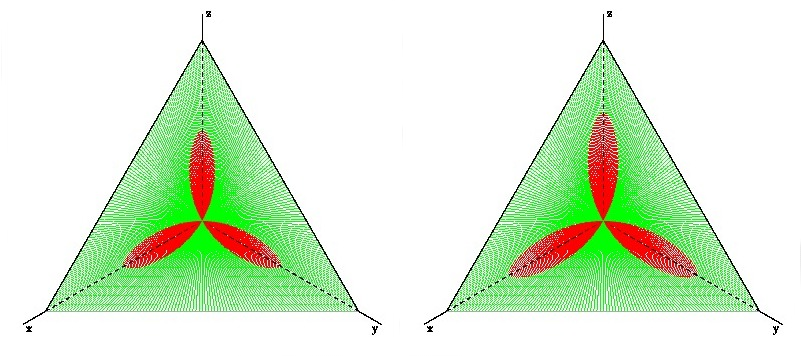
\includegraphics[width=\textwidth]{fleur-concat-edited.png}
      \caption{\footnotesize These two diagrams illustrate
        inequalities (\ref{eq:iengaech}) and (\ref{eq:feovaivo}). The
        former displays all points in red which violate
        \textsc{collinear horizon}, measured from the centre. The
        latter displays points in different colours whose orientation
        of asymmetry differs, measured from the centre. The two red
        sets are not the same, but there appears to be a relationship,
        one that ultimately I suspect to be due to the more basic
        property of asymmetry.}
      \label{fig:eeghoomo}
    \end{minipage}
  \end{flushright}
\end{figure}

Figure \ref{fig:eeghoomo} illustrates what I mean. Consider the
following two inequalities, where $M$ is represented by the centre
$m$ of the simplex with $m_{i}=1/n$ and $Y$ is an arbitrary
probability distribution with $X$ as the midpoint between $M$ and $Y$,
so $x_{i}=0.5(m_{i}+y_{i})$.

\begin{equation}
  \label{eq:dailoosu}
  \mbox{(i) }D_{\mbox{\tiny KL}}(Y,M)>D_{\mbox{\tiny KL}}(M,Y)\mbox{ and (ii) }D_{\mbox{\tiny KL}}(X,M)>D_{\mbox{\tiny KL}}(Y,X)
\end{equation}

In terms of coordinates, the inequalities reduce to ($H$ being the
Shannon entropy)

\begin{equation}
  \label{eq:iengaech}
\mbox{(i) }H(y)<\frac{1}{n}\sum\left(\log{}y_{i}\right)-\log\frac{1}{n^{2}}\mbox{ and}
\end{equation}

\begin{equation}
  \label{eq:feovaivo}
\mbox{(ii) }H(y)>\log\frac{4}{n}-\sum\left[\left(\frac{3}{2}y_{i}+\frac{1}{2n}\right)\log\left(y_{i}+\frac{1}{n}\right)\right].
\end{equation}

(i) is simply the case described in the next subsection for asymmetry
and illustrated on the bottom left of figure \ref{fig:concat}. (ii)
tells us how far from the midpoint I can go with a scenario where
$p=m,p'=q$ while violating \textsc{collinear horizon}. As illustrated
in figure \ref{fig:eeghoomo}, there may be a relationship between
asymmetry and \textsc{collinear horizon}.

\begin{figure}[H]
  \begin{flushright}
    \begin{minipage}[h]{\linewidth}
      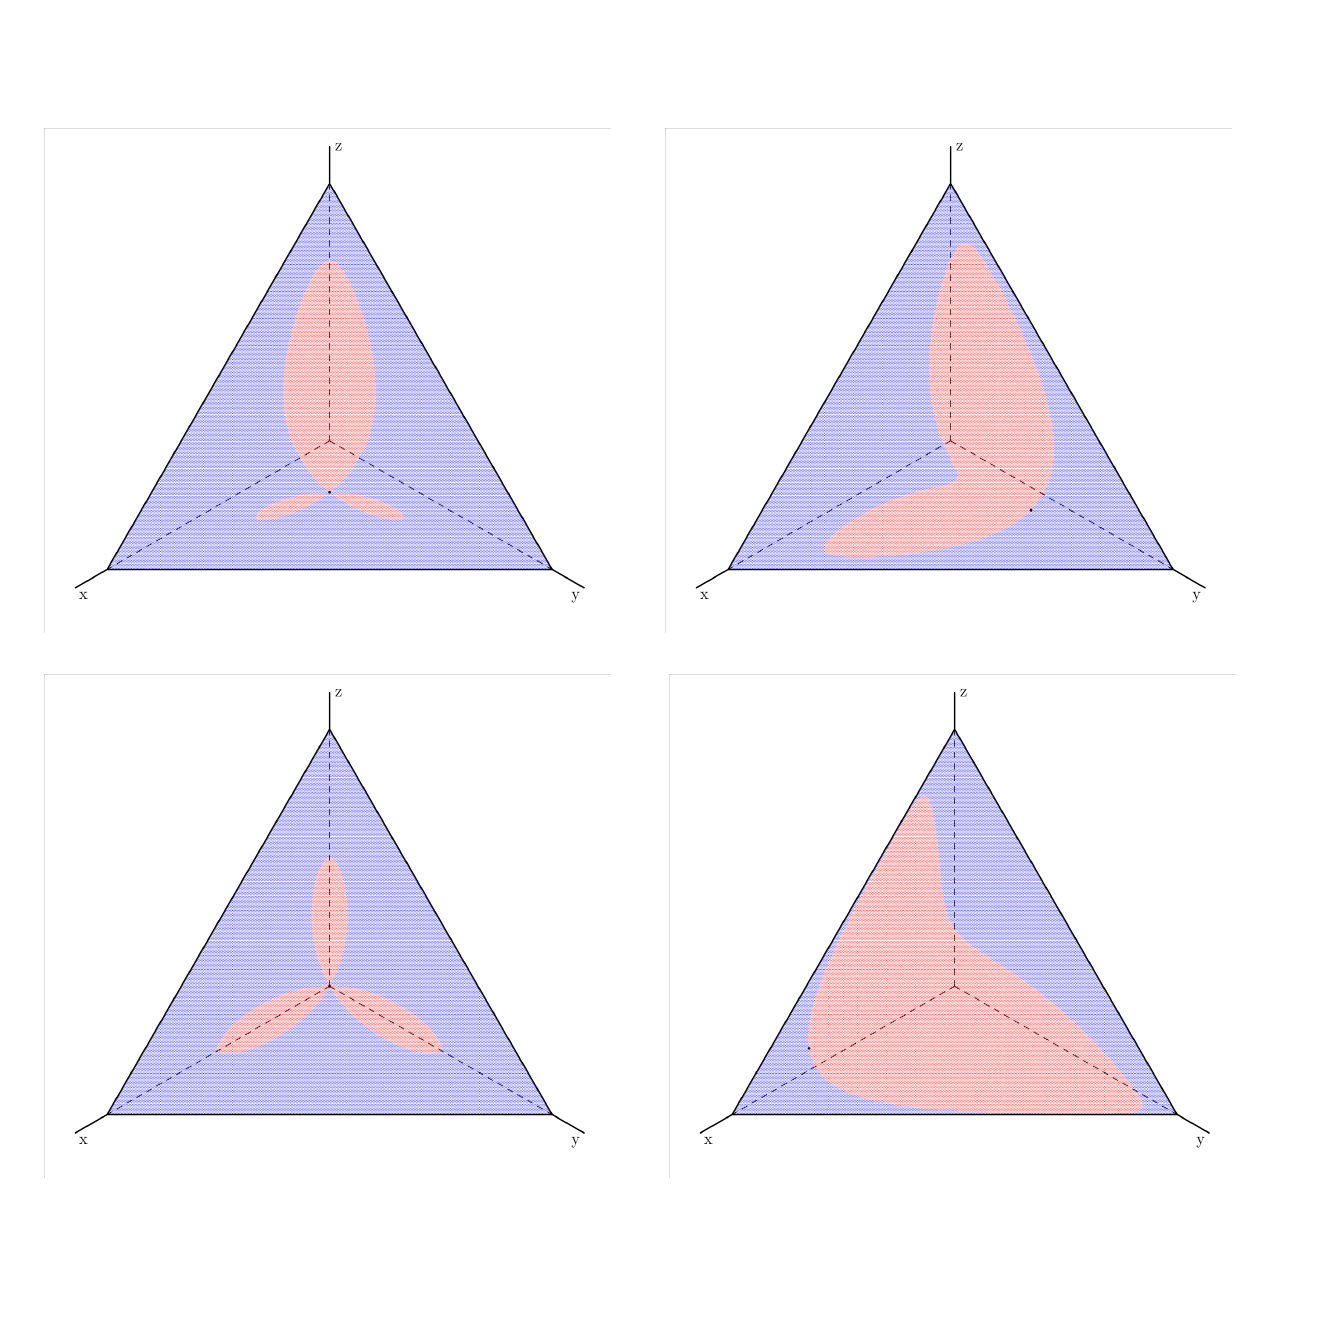
\includegraphics[width=\textwidth]{concat2.png}
      \caption{\footnotesize The partition (\ref{eq:sieruxis}) based
        on different values for $P$. From top left to bottom right,
        $P=(0.4,0.4,0.2); P=(0.242,0.604,0.154); P=(1/3,1/3,1/3);
        P=(0.741,0.087,0.172)$.
        Note that for the geometry of reason, the diagrams are
        trivial. The challenge for information theory is to explain
        the non-triviality of these diagrams epistemically without
        begging the question.}
      \label{fig:concat}
    \end{minipage}
  \end{flushright}
\end{figure}

It is not transparent what motivates information theory not only to
put probability distributions farther apart near the periphery, as
expected, but also near the centre. I lack the epistemic intuition
reflected in this behaviour. The next subsection on asymmetry deals
with this lack of epistemic intuition writ large.

\subsubsection{Transitivity of Asymmetry}
\label{subsubsec:Asymmetry}

Asymmetry presents a problem for the geometry of reason as well as for
information theory. For the geometry of reason, the problem is akin to
\textsc{continuity}. For information theory, the problem is the
non-trivial nature of the asymmetries it induces, which somehow need
to be reconnected to epistemic justification. I will consider this
problem in a moment, but first I will have a look at the problem for
the geometry of reason.

Extreme probabilities are special and create asymmetries in updating:
moving in direction from certainty to uncertainty is asymmetrical to
moving in direction from uncertainty to certainty. Geometry of
reason's metric topology, however, allows for no asymmetries.

\begin{example}[Extreme Asymmetry]
  \label{ex:extreme}
  Consider two cases where for case 1 the prior probabilities are
  $Y_{1}=(0.4,0.3,0.3)$ and the posterior probabilities are
  $Y_{1}'=(0,0.5,0.5)$; for case 2 the prior probabilities are
  reversed, so $Y_{2}=(0,0.5,0.5)$ and the posterior probabilities
  $Y_{2}'=(0.4,0.3,0.3)$.
\end{example}

Case 1 is a straightforward application of standard conditioning. Case
2 is more complicated: what does it take to raise a prior probability
of zero to a positive number? In terms of information theory, the
information required is infinite. Case 2 is also not compatible with
standard conditioning (at least not with what Alan H{\'a}jek calls the
ratio analysis of conditional probability, see \scite{7}{hajek03}{}).
The geometry of reason may want to solve this problem by signing on to
a version of regularity but is ill-advised to do so because LP
conditioning violates \textsc{regularity} independently.
% Happy kids, clean house, sanity: the hapless homemaker must pick two.
% The third remains elusive.
Continuity, a consistent view of regularity, and symmetry: the 
geometry of reason cannot consistently hold all three.

Now turn to information theory. Given the asymmetric similarity
measure of probability distributions that information theory requires
(the Kullback-Leibler divergence), a prior probability distribution
$P$ may be closer to a posterior probability distribution $Q$ than $Q$
is to $P$ if their roles (prior-posterior) are reversed. That is just
what we would expect. The problem is that there is another posterior
probability distribution $R$ where the situation is just the opposite:
prior $P$ is further away from posterior $R$ than prior $R$ is from
posterior $P$. And whether a probability distribution different from
$P$ is of the $Q$-type or of the $R$-type escapes any epistemic
intuition.

% For simplicity, let us consider probability distributions and their
% associated credence functions on an event space with three mutually
% exclusive and jointly comprehensive atoms
% $\Omega=\{\omega_{1},\omega_{2},\omega_{3}\}$.
The simplex $\mathbb{S}^{2}$ represents all the probability
distributions for trichotomy. Every point $p$ in $\mathbb{S}^{2}$
representing a probability distribution $P$ induces a partition on
$\mathbb{S}^{2}$ into points that are symmetric to $p$, positively
skew-symmetric to $p$, and negatively skew-symmetric to $p$ given the
topology of information theory.

In other words, if

\begin{equation}
  \label{eq:sksy}
  \Delta_{P}(P')=D_{\mbox{\tiny KL}}(P',P)-D_{\mbox{\tiny KL}}(P,P'),
\end{equation}

then, holding $P$ fixed, $\mathbb{S}^{2}$ is partitioned into three
regions,

\begin{equation}
  \label{eq:sieruxis}
  \Delta^{-1}(\mathbb{R}_{>0})\hspace{.5in}\Delta^{-1}(\mathbb{R}_{<0})\hspace{.5in}\Delta^{-1}(\{0\}).
\end{equation}

One could have a simple epistemic intuition such as \qnull{it takes
  less to update from a more uncertain probability distribution to a
  more certain probability distribution than the reverse direction,}
where the degree of certainty in a probability distribution is
measured by its entropy. This simple intuition accords with what we
said about extreme probabilities and it holds true for the asymmetric
distance measure defined by the Kullback-Leibler divergence in the
two-dimensional case where $\Omega$ has only two elements.

In higher-dimensional cases, however, the tripartite partition
(\ref{eq:sieruxis}) is non-trivial---some probability distributions
are of the $Q$-type, some are of the $R$-type, and it is difficult to
think of an epistemic distinction between them that does not already
presuppose information theory (see figure~\ref{fig:concat} for
illustration). The Legendre-Fenchel duality from
{\ubsection}~\ref{subsec:ohahpaiv} may be helpful, or else a more
coordinate-free approach using differential geometry. I do not know.

On any account of well-behaved and ill-behaved asymmetries, the
Kullback-Leibler divergence is ill-behaved. Of the four axioms as
listed by Ralph Kopperman for a distance measure $d$ (see
\scite{8}{kopperman88}{89}), the Kullback-Leibler divergence violates
both symmetry and triangularity, making it a \qnull{semi-quasimetric}:

\begin{enumerate}[(m1)]
\item $d(x,x)=0$ (self-similarity)
\item $d(x,z)\leq{}d(x,y)+d(y,z)$ (triangularity)
\item $d(x,y)=d(y,x)$ (symmetry)
\item $d(x,y)=0$ implies $x=y$ (separation)
\end{enumerate}

The Kullback-Leibler divergence not only violates symmetry and
triangularity, but also \textsc{transitivity of asymmetry}. For a
description of \textsc{transitivity of asymmetry} see \textbf{List B}.
For an example of it, consider

\begin{equation}
  \label{eq:transviol}
    P_{1}=\left(\frac{1}{2},\frac{1}{4},\frac{1}{4}\right)  \hspace{.5in}
    P_{2}=\left(\frac{1}{3},\frac{1}{3},\frac{1}{3}\right) \hspace{.5in}
    P_{3}=\left(\frac{2}{5},\frac{2}{5},\frac{1}{5}\right).
\end{equation}

In the terminology of \textsc{transitivity of asymmetry} in \textbf{List B},
$(P_{1},P_{2})$ is asymmetrically positive, and so is $(P_{2},P_{3})$.
The reasonable expectation is that $(P_{1},P_{3})$ is asymmetrically
positive by transitivity, but for the example in (\ref{eq:transviol})
it is asymmetrically negative.

How counterintuitive this is (epistemically and otherwise) is
demonstrated by the fact that in MDS (the multi-dimensional scaling of
distance relationships) almost all asymmetric distance relationships
under consideration are asymmetrically transitive in this sense, for
examples see international trade in \scite{7}{chino78}{}; journal
citation in \scite{7}{coombs64}{}; car switch in
\scite{7}{harshmanetal82}{}; telephone calls in
\scite{7}{harshmanlundy84}{}; interaction or input-output flow in
migration, economic activity, and social mobility in
\scite{7}{coxonetal82}{}; flight time between two cities in
\scite{8}{gentleman06}{191}; mutual intelligibility between Swedish
and Danish in \scite{8}{vanommenetal13}{193}; Tobler's wind model in
\scite{7}{tobler75}{}; and the cyclist lovingly hand-sketched in
\scite{8}{kopperman88}{91}.

This \qnull{ill behaviour} of information theory begs for explanation.
It would help, for example, to know that all reasonable
non-commutative difference measures used for updating are ill-behaved.
For a future research project, it would be interesting either to see
information theory debunked in favour of an alternative geometry (this
paper has demonstrated that this alternative will not be the geometry
of reason); or to see uniqueness results for the Kullback-Leibler
divergence to show that despite its ill behaviour the Kullback-Leibler
is the right asymmetric distance measure on which to base inference
and updating.

\section{Conclusion}
\label{sec:apaitahx}

% \begin{tabular}{|l|l|l|l|l|}\hline
%   \textbf{property} & \textbf{Brier score} & \textbf{Log score} & \textbf{other scores} & \textbf{annotation} \\ \hline
%   propriety & yes & yes & yes & commonly accepted \\ \hline
%   geometry & yes & no & no & implausible \\ \hline
%   information & no & yes & no & plausible \\ \hline
%   symmetry & yes & no & no & implausible \\ \hline
%   locality & no & yes & no & weakly plausible \\ \hline
%   horizon & no & long story & perhaps & plausible \\ \hline
%   sensitivity & yes & no & perhaps & implausible \\ \hline
%   conditioning & yes & yes & perhaps & plausible \\ \hline
%   reductio-resistance & no & yes & perhaps & plausible \\ \hline
%   univocal dominance & yes & yes & perhaps & implausible \\ \hline
% \end{tabular}

I have shown that the account provided by defenders of the geometry of
reason, such as Leitgeb, Pettigrew, or Selten, is indefensible. While
it is true that the scoring rule associated with the geometry of
reason, the Brier score, is unique in fulfilling a symmetry
requirement, I have shown both conceptually and by example that
asymmetry is preferable because it allows for greater sensitivity to
extreme probabilities. The Log score associated with information
theory fulfills the requirement to be sensitive to extremity and
therefore asymmetric. However, the Log score behaves oddly toward the
centre of probability distributions (for example, its asymmetry is not
transitive) and is in general an ill-behaved measure of divergence
(for example, it not only violates triangularity but does so in
egregious ways as demonstrated in the paper).

Both the geometry of reason and information theory are
well-established and highly integrated theories, with many interesting
results and various ways in which they have intuitive appeal. The
geometry of reason has in its favour that it makes use of our
geometric intuition as well as the substantial mathematical apparatus
that comes along with it. In a table in
{\ubsection}~\ref{subsec:ayudoosa} I have summarized, however, that
the geometry of reason fails several plausible requirements
(\textsc{information}, \textsc{locality}, \textsc{horizon},
\textsc{reductio-resistance}) and uniquely fulfills only implausible
requirements (\textsc{geometry}, \textsc{symmetry}).

A requirement that Pettigrew lists in favour of the geometry of
reason, \textsc{univocal dominance}, is fulfilled via
\textsc{symmetry}, but information theory also fulfills it via
\textsc{locality}, and the requirement itself is suspect (see
{\ubsection}~\ref{subsec:eemeingo}). Most significantly, besides the
violation of sensitivity to extremity, the geometry of reason does not
agree with intuitions that most of us have about updating. At the same
time, this is one of the major strengths of information theory. Both
standard conditioning (Bayesian conditioning) and Jeffrey conditioning
can be justified using information theory. Information theory licences
an updating method on affine constraints, the principle of minimum
cross-entropy, which generalizes both standard and Jeffrey
conditioning.

Information theory also gives us the entropy function we have come to
expect on the basis of Shannon's analysis of entropy in
\scite{7}{shannon48}{}. It fulfills Shannon's axioms, while the
entropy function associated with the geometry of reason fails them.
The work, however, is not complete. Further investigations may reveal
why information theory saddles us with a divergence function as
ill-behaved as the Kullback-Leibler divergence. I have introduced the
Legendre-Fenchel duality in {\ubsection}~\ref{subsec:ohahpaiv}, which
has potential to shed some light on this issue.

More promising yet is the use of differential geometry in the formal
theory of partial beliefs. This paper is still entrenched in thinking
of partial beliefs as parametrized by probabilities
$p_{i},i=1,{\ldots},n$. The geometry of reason is dedicated to this
entrenchment on principle. Information theory can hopefully escape it.
There are many other parameters that uniquely identify probability
distributions, for example
\begin{equation}
  \label{eq:eemaepie}
  \left(\ln\frac{p_{1}}{p_{n}},{\ldots},\ln\frac{p_{n-1}}{p_{n}}\right)^{\intercal}.
\end{equation}
Once a categorical distribution (corresponding to finite outcome
spaces) is parametrized this way, it joins the legion of other
distributions in the exponential family (normal, exponential, gamma,
chi-squared, beta, Dirichlet, Bernoulli, Poisson, Wishart, inverse
Wishart, geometric) and partakes in substantial results for these
distributions. The geometry of reason prevents us from pursuing these
fruitful abstractions by tying us to our geometric intuitions. Whether
information theory proves to be useful is a question for which I
eagerly await answers.

% \section{References}
% \label{refs}

% \nocite{*} 

% set bibtex bibliography to chicago style
% \bibliographystyle{chicago}

\bibliographystyle{ChicagoReedweb} 
\bibliography{bib-2902}

\end{document}
